
% Default to the notebook output style

    


% Inherit from the specified cell style.




    
\documentclass[11pt]{article}

    
    
    \usepackage[T1]{fontenc}
    % Nicer default font (+ math font) than Computer Modern for most use cases
    \usepackage{mathpazo}

    % Basic figure setup, for now with no caption control since it's done
    % automatically by Pandoc (which extracts ![](path) syntax from Markdown).
    \usepackage{graphicx}
    % We will generate all images so they have a width \maxwidth. This means
    % that they will get their normal width if they fit onto the page, but
    % are scaled down if they would overflow the margins.
    \makeatletter
    \def\maxwidth{\ifdim\Gin@nat@width>\linewidth\linewidth
    \else\Gin@nat@width\fi}
    \makeatother
    \let\Oldincludegraphics\includegraphics
    % Set max figure width to be 80% of text width, for now hardcoded.
    \renewcommand{\includegraphics}[1]{\Oldincludegraphics[width=.8\maxwidth]{#1}}
    % Ensure that by default, figures have no caption (until we provide a
    % proper Figure object with a Caption API and a way to capture that
    % in the conversion process - todo).
    \usepackage{caption}
    \DeclareCaptionLabelFormat{nolabel}{}
    \captionsetup{labelformat=nolabel}

    \usepackage{adjustbox} % Used to constrain images to a maximum size 
    \usepackage{xcolor} % Allow colors to be defined
    \usepackage{enumerate} % Needed for markdown enumerations to work
    \usepackage{geometry} % Used to adjust the document margins
    \usepackage{amsmath} % Equations
    \usepackage{amssymb} % Equations
    \usepackage{textcomp} % defines textquotesingle
    % Hack from http://tex.stackexchange.com/a/47451/13684:
    \AtBeginDocument{%
        \def\PYZsq{\textquotesingle}% Upright quotes in Pygmentized code
    }
    \usepackage{upquote} % Upright quotes for verbatim code
    \usepackage{eurosym} % defines \euro
    \usepackage[mathletters]{ucs} % Extended unicode (utf-8) support
    \usepackage[utf8x]{inputenc} % Allow utf-8 characters in the tex document
    \usepackage{fancyvrb} % verbatim replacement that allows latex
    \usepackage{grffile} % extends the file name processing of package graphics 
                         % to support a larger range 
    % The hyperref package gives us a pdf with properly built
    % internal navigation ('pdf bookmarks' for the table of contents,
    % internal cross-reference links, web links for URLs, etc.)
    \usepackage{hyperref}
    \usepackage{longtable} % longtable support required by pandoc >1.10
    \usepackage{booktabs}  % table support for pandoc > 1.12.2
    \usepackage[inline]{enumitem} % IRkernel/repr support (it uses the enumerate* environment)
    \usepackage[normalem]{ulem} % ulem is needed to support strikethroughs (\sout)
                                % normalem makes italics be italics, not underlines
    

    
    
    % Colors for the hyperref package
    \definecolor{urlcolor}{rgb}{0,.145,.698}
    \definecolor{linkcolor}{rgb}{.71,0.21,0.01}
    \definecolor{citecolor}{rgb}{.12,.54,.11}

    % ANSI colors
    \definecolor{ansi-black}{HTML}{3E424D}
    \definecolor{ansi-black-intense}{HTML}{282C36}
    \definecolor{ansi-red}{HTML}{E75C58}
    \definecolor{ansi-red-intense}{HTML}{B22B31}
    \definecolor{ansi-green}{HTML}{00A250}
    \definecolor{ansi-green-intense}{HTML}{007427}
    \definecolor{ansi-yellow}{HTML}{DDB62B}
    \definecolor{ansi-yellow-intense}{HTML}{B27D12}
    \definecolor{ansi-blue}{HTML}{208FFB}
    \definecolor{ansi-blue-intense}{HTML}{0065CA}
    \definecolor{ansi-magenta}{HTML}{D160C4}
    \definecolor{ansi-magenta-intense}{HTML}{A03196}
    \definecolor{ansi-cyan}{HTML}{60C6C8}
    \definecolor{ansi-cyan-intense}{HTML}{258F8F}
    \definecolor{ansi-white}{HTML}{C5C1B4}
    \definecolor{ansi-white-intense}{HTML}{A1A6B2}

    % commands and environments needed by pandoc snippets
    % extracted from the output of `pandoc -s`
    \providecommand{\tightlist}{%
      \setlength{\itemsep}{0pt}\setlength{\parskip}{0pt}}
    \DefineVerbatimEnvironment{Highlighting}{Verbatim}{commandchars=\\\{\}}
    % Add ',fontsize=\small' for more characters per line
    \newenvironment{Shaded}{}{}
    \newcommand{\KeywordTok}[1]{\textcolor[rgb]{0.00,0.44,0.13}{\textbf{{#1}}}}
    \newcommand{\DataTypeTok}[1]{\textcolor[rgb]{0.56,0.13,0.00}{{#1}}}
    \newcommand{\DecValTok}[1]{\textcolor[rgb]{0.25,0.63,0.44}{{#1}}}
    \newcommand{\BaseNTok}[1]{\textcolor[rgb]{0.25,0.63,0.44}{{#1}}}
    \newcommand{\FloatTok}[1]{\textcolor[rgb]{0.25,0.63,0.44}{{#1}}}
    \newcommand{\CharTok}[1]{\textcolor[rgb]{0.25,0.44,0.63}{{#1}}}
    \newcommand{\StringTok}[1]{\textcolor[rgb]{0.25,0.44,0.63}{{#1}}}
    \newcommand{\CommentTok}[1]{\textcolor[rgb]{0.38,0.63,0.69}{\textit{{#1}}}}
    \newcommand{\OtherTok}[1]{\textcolor[rgb]{0.00,0.44,0.13}{{#1}}}
    \newcommand{\AlertTok}[1]{\textcolor[rgb]{1.00,0.00,0.00}{\textbf{{#1}}}}
    \newcommand{\FunctionTok}[1]{\textcolor[rgb]{0.02,0.16,0.49}{{#1}}}
    \newcommand{\RegionMarkerTok}[1]{{#1}}
    \newcommand{\ErrorTok}[1]{\textcolor[rgb]{1.00,0.00,0.00}{\textbf{{#1}}}}
    \newcommand{\NormalTok}[1]{{#1}}
    
    % Additional commands for more recent versions of Pandoc
    \newcommand{\ConstantTok}[1]{\textcolor[rgb]{0.53,0.00,0.00}{{#1}}}
    \newcommand{\SpecialCharTok}[1]{\textcolor[rgb]{0.25,0.44,0.63}{{#1}}}
    \newcommand{\VerbatimStringTok}[1]{\textcolor[rgb]{0.25,0.44,0.63}{{#1}}}
    \newcommand{\SpecialStringTok}[1]{\textcolor[rgb]{0.73,0.40,0.53}{{#1}}}
    \newcommand{\ImportTok}[1]{{#1}}
    \newcommand{\DocumentationTok}[1]{\textcolor[rgb]{0.73,0.13,0.13}{\textit{{#1}}}}
    \newcommand{\AnnotationTok}[1]{\textcolor[rgb]{0.38,0.63,0.69}{\textbf{\textit{{#1}}}}}
    \newcommand{\CommentVarTok}[1]{\textcolor[rgb]{0.38,0.63,0.69}{\textbf{\textit{{#1}}}}}
    \newcommand{\VariableTok}[1]{\textcolor[rgb]{0.10,0.09,0.49}{{#1}}}
    \newcommand{\ControlFlowTok}[1]{\textcolor[rgb]{0.00,0.44,0.13}{\textbf{{#1}}}}
    \newcommand{\OperatorTok}[1]{\textcolor[rgb]{0.40,0.40,0.40}{{#1}}}
    \newcommand{\BuiltInTok}[1]{{#1}}
    \newcommand{\ExtensionTok}[1]{{#1}}
    \newcommand{\PreprocessorTok}[1]{\textcolor[rgb]{0.74,0.48,0.00}{{#1}}}
    \newcommand{\AttributeTok}[1]{\textcolor[rgb]{0.49,0.56,0.16}{{#1}}}
    \newcommand{\InformationTok}[1]{\textcolor[rgb]{0.38,0.63,0.69}{\textbf{\textit{{#1}}}}}
    \newcommand{\WarningTok}[1]{\textcolor[rgb]{0.38,0.63,0.69}{\textbf{\textit{{#1}}}}}
    
    
    % Define a nice break command that doesn't care if a line doesn't already
    % exist.
    \def\br{\hspace*{\fill} \\* }
    % Math Jax compatability definitions
    \def\gt{>}
    \def\lt{<}
    % Document parameters
    \title{ex3}
    
    
    

    % Pygments definitions
    
\makeatletter
\def\PY@reset{\let\PY@it=\relax \let\PY@bf=\relax%
    \let\PY@ul=\relax \let\PY@tc=\relax%
    \let\PY@bc=\relax \let\PY@ff=\relax}
\def\PY@tok#1{\csname PY@tok@#1\endcsname}
\def\PY@toks#1+{\ifx\relax#1\empty\else%
    \PY@tok{#1}\expandafter\PY@toks\fi}
\def\PY@do#1{\PY@bc{\PY@tc{\PY@ul{%
    \PY@it{\PY@bf{\PY@ff{#1}}}}}}}
\def\PY#1#2{\PY@reset\PY@toks#1+\relax+\PY@do{#2}}

\expandafter\def\csname PY@tok@w\endcsname{\def\PY@tc##1{\textcolor[rgb]{0.73,0.73,0.73}{##1}}}
\expandafter\def\csname PY@tok@c\endcsname{\let\PY@it=\textit\def\PY@tc##1{\textcolor[rgb]{0.25,0.50,0.50}{##1}}}
\expandafter\def\csname PY@tok@cp\endcsname{\def\PY@tc##1{\textcolor[rgb]{0.74,0.48,0.00}{##1}}}
\expandafter\def\csname PY@tok@k\endcsname{\let\PY@bf=\textbf\def\PY@tc##1{\textcolor[rgb]{0.00,0.50,0.00}{##1}}}
\expandafter\def\csname PY@tok@kp\endcsname{\def\PY@tc##1{\textcolor[rgb]{0.00,0.50,0.00}{##1}}}
\expandafter\def\csname PY@tok@kt\endcsname{\def\PY@tc##1{\textcolor[rgb]{0.69,0.00,0.25}{##1}}}
\expandafter\def\csname PY@tok@o\endcsname{\def\PY@tc##1{\textcolor[rgb]{0.40,0.40,0.40}{##1}}}
\expandafter\def\csname PY@tok@ow\endcsname{\let\PY@bf=\textbf\def\PY@tc##1{\textcolor[rgb]{0.67,0.13,1.00}{##1}}}
\expandafter\def\csname PY@tok@nb\endcsname{\def\PY@tc##1{\textcolor[rgb]{0.00,0.50,0.00}{##1}}}
\expandafter\def\csname PY@tok@nf\endcsname{\def\PY@tc##1{\textcolor[rgb]{0.00,0.00,1.00}{##1}}}
\expandafter\def\csname PY@tok@nc\endcsname{\let\PY@bf=\textbf\def\PY@tc##1{\textcolor[rgb]{0.00,0.00,1.00}{##1}}}
\expandafter\def\csname PY@tok@nn\endcsname{\let\PY@bf=\textbf\def\PY@tc##1{\textcolor[rgb]{0.00,0.00,1.00}{##1}}}
\expandafter\def\csname PY@tok@ne\endcsname{\let\PY@bf=\textbf\def\PY@tc##1{\textcolor[rgb]{0.82,0.25,0.23}{##1}}}
\expandafter\def\csname PY@tok@nv\endcsname{\def\PY@tc##1{\textcolor[rgb]{0.10,0.09,0.49}{##1}}}
\expandafter\def\csname PY@tok@no\endcsname{\def\PY@tc##1{\textcolor[rgb]{0.53,0.00,0.00}{##1}}}
\expandafter\def\csname PY@tok@nl\endcsname{\def\PY@tc##1{\textcolor[rgb]{0.63,0.63,0.00}{##1}}}
\expandafter\def\csname PY@tok@ni\endcsname{\let\PY@bf=\textbf\def\PY@tc##1{\textcolor[rgb]{0.60,0.60,0.60}{##1}}}
\expandafter\def\csname PY@tok@na\endcsname{\def\PY@tc##1{\textcolor[rgb]{0.49,0.56,0.16}{##1}}}
\expandafter\def\csname PY@tok@nt\endcsname{\let\PY@bf=\textbf\def\PY@tc##1{\textcolor[rgb]{0.00,0.50,0.00}{##1}}}
\expandafter\def\csname PY@tok@nd\endcsname{\def\PY@tc##1{\textcolor[rgb]{0.67,0.13,1.00}{##1}}}
\expandafter\def\csname PY@tok@s\endcsname{\def\PY@tc##1{\textcolor[rgb]{0.73,0.13,0.13}{##1}}}
\expandafter\def\csname PY@tok@sd\endcsname{\let\PY@it=\textit\def\PY@tc##1{\textcolor[rgb]{0.73,0.13,0.13}{##1}}}
\expandafter\def\csname PY@tok@si\endcsname{\let\PY@bf=\textbf\def\PY@tc##1{\textcolor[rgb]{0.73,0.40,0.53}{##1}}}
\expandafter\def\csname PY@tok@se\endcsname{\let\PY@bf=\textbf\def\PY@tc##1{\textcolor[rgb]{0.73,0.40,0.13}{##1}}}
\expandafter\def\csname PY@tok@sr\endcsname{\def\PY@tc##1{\textcolor[rgb]{0.73,0.40,0.53}{##1}}}
\expandafter\def\csname PY@tok@ss\endcsname{\def\PY@tc##1{\textcolor[rgb]{0.10,0.09,0.49}{##1}}}
\expandafter\def\csname PY@tok@sx\endcsname{\def\PY@tc##1{\textcolor[rgb]{0.00,0.50,0.00}{##1}}}
\expandafter\def\csname PY@tok@m\endcsname{\def\PY@tc##1{\textcolor[rgb]{0.40,0.40,0.40}{##1}}}
\expandafter\def\csname PY@tok@gh\endcsname{\let\PY@bf=\textbf\def\PY@tc##1{\textcolor[rgb]{0.00,0.00,0.50}{##1}}}
\expandafter\def\csname PY@tok@gu\endcsname{\let\PY@bf=\textbf\def\PY@tc##1{\textcolor[rgb]{0.50,0.00,0.50}{##1}}}
\expandafter\def\csname PY@tok@gd\endcsname{\def\PY@tc##1{\textcolor[rgb]{0.63,0.00,0.00}{##1}}}
\expandafter\def\csname PY@tok@gi\endcsname{\def\PY@tc##1{\textcolor[rgb]{0.00,0.63,0.00}{##1}}}
\expandafter\def\csname PY@tok@gr\endcsname{\def\PY@tc##1{\textcolor[rgb]{1.00,0.00,0.00}{##1}}}
\expandafter\def\csname PY@tok@ge\endcsname{\let\PY@it=\textit}
\expandafter\def\csname PY@tok@gs\endcsname{\let\PY@bf=\textbf}
\expandafter\def\csname PY@tok@gp\endcsname{\let\PY@bf=\textbf\def\PY@tc##1{\textcolor[rgb]{0.00,0.00,0.50}{##1}}}
\expandafter\def\csname PY@tok@go\endcsname{\def\PY@tc##1{\textcolor[rgb]{0.53,0.53,0.53}{##1}}}
\expandafter\def\csname PY@tok@gt\endcsname{\def\PY@tc##1{\textcolor[rgb]{0.00,0.27,0.87}{##1}}}
\expandafter\def\csname PY@tok@err\endcsname{\def\PY@bc##1{\setlength{\fboxsep}{0pt}\fcolorbox[rgb]{1.00,0.00,0.00}{1,1,1}{\strut ##1}}}
\expandafter\def\csname PY@tok@kc\endcsname{\let\PY@bf=\textbf\def\PY@tc##1{\textcolor[rgb]{0.00,0.50,0.00}{##1}}}
\expandafter\def\csname PY@tok@kd\endcsname{\let\PY@bf=\textbf\def\PY@tc##1{\textcolor[rgb]{0.00,0.50,0.00}{##1}}}
\expandafter\def\csname PY@tok@kn\endcsname{\let\PY@bf=\textbf\def\PY@tc##1{\textcolor[rgb]{0.00,0.50,0.00}{##1}}}
\expandafter\def\csname PY@tok@kr\endcsname{\let\PY@bf=\textbf\def\PY@tc##1{\textcolor[rgb]{0.00,0.50,0.00}{##1}}}
\expandafter\def\csname PY@tok@bp\endcsname{\def\PY@tc##1{\textcolor[rgb]{0.00,0.50,0.00}{##1}}}
\expandafter\def\csname PY@tok@fm\endcsname{\def\PY@tc##1{\textcolor[rgb]{0.00,0.00,1.00}{##1}}}
\expandafter\def\csname PY@tok@vc\endcsname{\def\PY@tc##1{\textcolor[rgb]{0.10,0.09,0.49}{##1}}}
\expandafter\def\csname PY@tok@vg\endcsname{\def\PY@tc##1{\textcolor[rgb]{0.10,0.09,0.49}{##1}}}
\expandafter\def\csname PY@tok@vi\endcsname{\def\PY@tc##1{\textcolor[rgb]{0.10,0.09,0.49}{##1}}}
\expandafter\def\csname PY@tok@vm\endcsname{\def\PY@tc##1{\textcolor[rgb]{0.10,0.09,0.49}{##1}}}
\expandafter\def\csname PY@tok@sa\endcsname{\def\PY@tc##1{\textcolor[rgb]{0.73,0.13,0.13}{##1}}}
\expandafter\def\csname PY@tok@sb\endcsname{\def\PY@tc##1{\textcolor[rgb]{0.73,0.13,0.13}{##1}}}
\expandafter\def\csname PY@tok@sc\endcsname{\def\PY@tc##1{\textcolor[rgb]{0.73,0.13,0.13}{##1}}}
\expandafter\def\csname PY@tok@dl\endcsname{\def\PY@tc##1{\textcolor[rgb]{0.73,0.13,0.13}{##1}}}
\expandafter\def\csname PY@tok@s2\endcsname{\def\PY@tc##1{\textcolor[rgb]{0.73,0.13,0.13}{##1}}}
\expandafter\def\csname PY@tok@sh\endcsname{\def\PY@tc##1{\textcolor[rgb]{0.73,0.13,0.13}{##1}}}
\expandafter\def\csname PY@tok@s1\endcsname{\def\PY@tc##1{\textcolor[rgb]{0.73,0.13,0.13}{##1}}}
\expandafter\def\csname PY@tok@mb\endcsname{\def\PY@tc##1{\textcolor[rgb]{0.40,0.40,0.40}{##1}}}
\expandafter\def\csname PY@tok@mf\endcsname{\def\PY@tc##1{\textcolor[rgb]{0.40,0.40,0.40}{##1}}}
\expandafter\def\csname PY@tok@mh\endcsname{\def\PY@tc##1{\textcolor[rgb]{0.40,0.40,0.40}{##1}}}
\expandafter\def\csname PY@tok@mi\endcsname{\def\PY@tc##1{\textcolor[rgb]{0.40,0.40,0.40}{##1}}}
\expandafter\def\csname PY@tok@il\endcsname{\def\PY@tc##1{\textcolor[rgb]{0.40,0.40,0.40}{##1}}}
\expandafter\def\csname PY@tok@mo\endcsname{\def\PY@tc##1{\textcolor[rgb]{0.40,0.40,0.40}{##1}}}
\expandafter\def\csname PY@tok@ch\endcsname{\let\PY@it=\textit\def\PY@tc##1{\textcolor[rgb]{0.25,0.50,0.50}{##1}}}
\expandafter\def\csname PY@tok@cm\endcsname{\let\PY@it=\textit\def\PY@tc##1{\textcolor[rgb]{0.25,0.50,0.50}{##1}}}
\expandafter\def\csname PY@tok@cpf\endcsname{\let\PY@it=\textit\def\PY@tc##1{\textcolor[rgb]{0.25,0.50,0.50}{##1}}}
\expandafter\def\csname PY@tok@c1\endcsname{\let\PY@it=\textit\def\PY@tc##1{\textcolor[rgb]{0.25,0.50,0.50}{##1}}}
\expandafter\def\csname PY@tok@cs\endcsname{\let\PY@it=\textit\def\PY@tc##1{\textcolor[rgb]{0.25,0.50,0.50}{##1}}}

\def\PYZbs{\char`\\}
\def\PYZus{\char`\_}
\def\PYZob{\char`\{}
\def\PYZcb{\char`\}}
\def\PYZca{\char`\^}
\def\PYZam{\char`\&}
\def\PYZlt{\char`\<}
\def\PYZgt{\char`\>}
\def\PYZsh{\char`\#}
\def\PYZpc{\char`\%}
\def\PYZdl{\char`\$}
\def\PYZhy{\char`\-}
\def\PYZsq{\char`\'}
\def\PYZdq{\char`\"}
\def\PYZti{\char`\~}
% for compatibility with earlier versions
\def\PYZat{@}
\def\PYZlb{[}
\def\PYZrb{]}
\makeatother


    % Exact colors from NB
    \definecolor{incolor}{rgb}{0.0, 0.0, 0.5}
    \definecolor{outcolor}{rgb}{0.545, 0.0, 0.0}



    
    % Prevent overflowing lines due to hard-to-break entities
    \sloppy 
    % Setup hyperref package
    \hypersetup{
      breaklinks=true,  % so long urls are correctly broken across lines
      colorlinks=true,
      urlcolor=urlcolor,
      linkcolor=linkcolor,
      citecolor=citecolor,
      }
    % Slightly bigger margins than the latex defaults
    
    \geometry{verbose,tmargin=1in,bmargin=1in,lmargin=1in,rmargin=1in}
    
    

    \begin{document}
    
    
    \maketitle
    
    

    
    \hypertarget{correlations}{%
\section{Correlations}\label{correlations}}

    \begin{Verbatim}[commandchars=\\\{\}]
{\color{incolor}In [{\color{incolor}20}]:} \PY{k+kn}{from} \PY{n+nn}{scipy}\PY{n+nn}{.}\PY{n+nn}{stats} \PY{k}{import} \PY{n}{pearsonr}
         \PY{k+kn}{from} \PY{n+nn}{tabulate} \PY{k}{import} \PY{n}{tabulate}
         \PY{k+kn}{import} \PY{n+nn}{matplotlib}\PY{n+nn}{.}\PY{n+nn}{pyplot} \PY{k}{as} \PY{n+nn}{plt}
         \PY{k+kn}{from} \PY{n+nn}{random} \PY{k}{import} \PY{n}{random}
         
         \PY{n}{x} \PY{o}{=} \PY{p}{[}\PY{n+nb}{round}\PY{p}{(}\PY{n}{random}\PY{p}{(}\PY{p}{)}\PY{p}{,} \PY{l+m+mi}{2}\PY{p}{)} \PY{o}{*} \PY{l+m+mi}{5} \PY{k}{for} \PY{n}{\PYZus{}} \PY{o+ow}{in} \PY{n+nb}{range}\PY{p}{(}\PY{l+m+mi}{49}\PY{p}{)}\PY{p}{]} \PY{o}{+} \PY{p}{[}\PY{l+m+mi}{100}\PY{p}{]}
         \PY{n}{y} \PY{o}{=} \PY{p}{[}\PY{n+nb}{round}\PY{p}{(}\PY{n}{random}\PY{p}{(}\PY{p}{)}\PY{p}{,} \PY{l+m+mi}{2}\PY{p}{)} \PY{o}{*} \PY{l+m+mi}{5} \PY{k}{for} \PY{n}{\PYZus{}} \PY{o+ow}{in} \PY{n+nb}{range}\PY{p}{(}\PY{l+m+mi}{49}\PY{p}{)}\PY{p}{]} \PY{o}{+} \PY{p}{[}\PY{l+m+mi}{100}\PY{p}{]}
         
         \PY{n}{full\PYZus{}pearson} \PY{o}{=} \PY{n}{pearsonr}\PY{p}{(}\PY{n}{x}\PY{p}{,} \PY{n}{y}\PY{p}{)}\PY{p}{[}\PY{l+m+mi}{0}\PY{p}{]}
         \PY{n}{n1\PYZus{}pearson} \PY{o}{=} \PY{n}{pearsonr}\PY{p}{(}\PY{n}{x}\PY{p}{[}\PY{p}{:}\PY{o}{\PYZhy{}}\PY{l+m+mi}{1}\PY{p}{]}\PY{p}{,} \PY{n}{y}\PY{p}{[}\PY{p}{:}\PY{o}{\PYZhy{}}\PY{l+m+mi}{1}\PY{p}{]}\PY{p}{)}\PY{p}{[}\PY{l+m+mi}{0}\PY{p}{]}
         \PY{n+nb}{print} \PY{p}{(}\PY{l+s+s2}{\PYZdq{}}\PY{l+s+s2}{Data in which the Pearson(x,y)\PYZgt{}0.9 but where n\PYZhy{}1 points can be selected so that for the vectors restricted to those we have Pearson correlation \PYZlt{}0.1}\PY{l+s+se}{\PYZbs{}n}\PY{l+s+s2}{\PYZdq{}}\PY{p}{)}
         \PY{n+nb}{print} \PY{p}{(}\PY{n}{tabulate}\PY{p}{(}\PY{n}{np}\PY{o}{.}\PY{n}{column\PYZus{}stack}\PY{p}{(}\PY{p}{(}\PY{n}{x}\PY{p}{,}\PY{n}{y}\PY{p}{)}\PY{p}{)}\PY{p}{,} \PY{n}{headers}\PY{o}{=}\PY{p}{[}\PY{l+s+s1}{\PYZsq{}}\PY{l+s+s1}{X}\PY{l+s+s1}{\PYZsq{}}\PY{p}{,} \PY{l+s+s1}{\PYZsq{}}\PY{l+s+s1}{Y}\PY{l+s+s1}{\PYZsq{}}\PY{p}{]}\PY{p}{)}\PY{p}{)}
         
         \PY{n}{plt}\PY{o}{.}\PY{n}{scatter}\PY{p}{(}\PY{n}{x}\PY{p}{,} \PY{n}{y}\PY{p}{,} \PY{n}{marker}\PY{o}{=}\PY{l+s+s1}{\PYZsq{}}\PY{l+s+s1}{x}\PY{l+s+s1}{\PYZsq{}}\PY{p}{)}
         \PY{n}{plt}\PY{o}{.}\PY{n}{xlabel}\PY{p}{(}\PY{l+s+s1}{\PYZsq{}}\PY{l+s+s1}{x}\PY{l+s+s1}{\PYZsq{}}\PY{p}{)}
         \PY{n}{plt}\PY{o}{.}\PY{n}{ylabel}\PY{p}{(}\PY{l+s+s1}{\PYZsq{}}\PY{l+s+s1}{y}\PY{l+s+s1}{\PYZsq{}}\PY{p}{)}
         \PY{n}{plt}\PY{o}{.}\PY{n}{title}\PY{p}{(}\PY{l+s+sa}{r}\PY{l+s+s1}{\PYZsq{}}\PY{l+s+s1}{\PYZdl{}Pearson=}\PY{l+s+si}{\PYZob{}\PYZcb{}}\PY{l+s+s1}{\PYZdl{}, \PYZdl{}Pearson[n\PYZhy{}1]=}\PY{l+s+si}{\PYZob{}\PYZcb{}}\PY{l+s+s1}{\PYZdl{}}\PY{l+s+s1}{\PYZsq{}}\PY{o}{.}\PY{n}{format}\PY{p}{(}\PY{n+nb}{round}\PY{p}{(}\PY{n}{full\PYZus{}pearson}\PY{p}{,} \PY{l+m+mi}{4}\PY{p}{)}\PY{p}{,} \PY{n+nb}{round}\PY{p}{(}\PY{n}{n1\PYZus{}pearson}\PY{p}{,} \PY{l+m+mi}{4}\PY{p}{)}\PY{p}{)}\PY{p}{)}
         \PY{n}{plt}\PY{o}{.}\PY{n}{show}\PY{p}{(}\PY{p}{)}
\end{Verbatim}


    \begin{Verbatim}[commandchars=\\\{\}]
Data in which the Pearson(x,y)>0.9 but where n-1 points can be selected so that for the vectors restricted to those we have Pearson correlation <0.1

     X       Y
------  ------
  0.8     1.4
  0.95    2.4
  2.75    4.1
  4.35    1.95
  1.05    2.35
  4.75    2.8
  3.75    4.5
  3.3     0.8
  4       4.25
  3.75    2.6
  2       4.3
  2.4     0.4
  0.65    3.35
  4.25    2.1
  2.3     3.8
  3.5     4.3
  1       1
  3.4     2.25
  2.2     1.1
  3.1     3.95
  2.35    0.55
  4.6     4.7
  2       1.65
  1.7     1.2
  4.45    0.7
  4.1     3.75
  4.35    0.4
  3.85    2.65
  0.7     1.8
  4       0.85
  1.8     2.85
  2.2     0.5
  3.4     3.95
  0.3     1.55
  4.1     2.2
  1.4     4.55
  2.85    5
  2.65    4.05
  3.45    1.5
  1.45    1
  1.6     2.55
  2.05    4.45
  0.05    2.1
  0.65    4.75
  4.25    3.4
  0.3     0.5
  1.6     3.15
  2.8     4.7
  4.95    4.25
100     100

    \end{Verbatim}

    \begin{center}
    \adjustimage{max size={0.9\linewidth}{0.9\paperheight}}{output_1_1.png}
    \end{center}
    { \hspace*{\fill} \\}
    
    \begin{Verbatim}[commandchars=\\\{\}]
{\color{incolor}In [{\color{incolor}21}]:} \PY{k+kn}{from} \PY{n+nn}{scipy}\PY{n+nn}{.}\PY{n+nn}{stats} \PY{k}{import} \PY{n}{spearmanr}\PY{p}{,} \PY{n}{kendalltau}\PY{p}{,} \PY{n}{rankdata}
         \PY{k+kn}{import} \PY{n+nn}{matplotlib}\PY{n+nn}{.}\PY{n+nn}{pyplot} \PY{k}{as} \PY{n+nn}{plt}
         \PY{k+kn}{from} \PY{n+nn}{random} \PY{k}{import} \PY{n}{random}
         \PY{k+kn}{from} \PY{n+nn}{pprint} \PY{k}{import} \PY{n}{pprint}
         \PY{k+kn}{from} \PY{n+nn}{tabulate} \PY{k}{import} \PY{n}{tabulate}
         \PY{k+kn}{import} \PY{n+nn}{numpy} \PY{k}{as} \PY{n+nn}{np}
         
         
         \PY{k}{def} \PY{n+nf}{kendall\PYZus{}tau}\PY{p}{(}\PY{n}{a}\PY{p}{,} \PY{n}{b}\PY{p}{)}\PY{p}{:}
             \PY{k}{return} \PY{n}{kendalltau}\PY{p}{(}\PY{n}{rankdata}\PY{p}{(}\PY{n}{a}\PY{p}{)}\PY{p}{,} \PY{n}{rankdata}\PY{p}{(}\PY{n}{b}\PY{p}{)}\PY{p}{)}
         
         \PY{n}{xs} \PY{o}{=} \PY{n+nb}{range}\PY{p}{(}\PY{l+m+mi}{50}\PY{p}{)}
         \PY{n}{ys} \PY{o}{=} \PY{n+nb}{list}\PY{p}{(}\PY{n+nb}{range}\PY{p}{(}\PY{l+m+mi}{25}\PY{p}{,}\PY{l+m+mi}{50}\PY{p}{)}\PY{p}{)} \PY{o}{+} \PY{n+nb}{list}\PY{p}{(}\PY{n+nb}{range}\PY{p}{(}\PY{l+m+mi}{25}\PY{p}{)}\PY{p}{)}
         
         \PY{n}{tau} \PY{o}{=} \PY{n}{kendalltau}\PY{p}{(}\PY{n}{xs}\PY{p}{,} \PY{n}{ys}\PY{p}{)}
         \PY{n}{rho} \PY{o}{=} \PY{n}{spearmanr}\PY{p}{(}\PY{n}{xs}\PY{p}{,} \PY{n}{ys}\PY{p}{)}
            
         \PY{n+nb}{print} \PY{p}{(}\PY{l+s+s2}{\PYZdq{}}\PY{l+s+s2}{Data with τ(x,y) \PYZgt{} ρ(x,y) + 0.4}\PY{l+s+se}{\PYZbs{}n}\PY{l+s+s2}{\PYZdq{}}\PY{p}{)}
         \PY{n+nb}{print} \PY{p}{(}\PY{n}{tabulate}\PY{p}{(}\PY{n}{np}\PY{o}{.}\PY{n}{column\PYZus{}stack}\PY{p}{(}\PY{p}{(}\PY{n}{xs}\PY{p}{,}\PY{n}{ys}\PY{p}{)}\PY{p}{)}\PY{p}{,} \PY{n}{headers}\PY{o}{=}\PY{p}{[}\PY{l+s+s1}{\PYZsq{}}\PY{l+s+s1}{X}\PY{l+s+s1}{\PYZsq{}}\PY{p}{,} \PY{l+s+s1}{\PYZsq{}}\PY{l+s+s1}{Y}\PY{l+s+s1}{\PYZsq{}}\PY{p}{]}\PY{p}{)}\PY{p}{)}
         
         \PY{n}{plt}\PY{o}{.}\PY{n}{rc}\PY{p}{(}\PY{l+s+s1}{\PYZsq{}}\PY{l+s+s1}{text}\PY{l+s+s1}{\PYZsq{}}\PY{p}{)}
         \PY{n}{plt}\PY{o}{.}\PY{n}{scatter}\PY{p}{(}\PY{n}{xs}\PY{p}{,} \PY{n}{ys}\PY{p}{,} \PY{n}{marker}\PY{o}{=}\PY{l+s+s1}{\PYZsq{}}\PY{l+s+s1}{x}\PY{l+s+s1}{\PYZsq{}}\PY{p}{)}
         \PY{n}{plt}\PY{o}{.}\PY{n}{xlabel}\PY{p}{(}\PY{l+s+s1}{\PYZsq{}}\PY{l+s+s1}{x}\PY{l+s+s1}{\PYZsq{}}\PY{p}{)}
         \PY{n}{plt}\PY{o}{.}\PY{n}{ylabel}\PY{p}{(}\PY{l+s+s1}{\PYZsq{}}\PY{l+s+s1}{y}\PY{l+s+s1}{\PYZsq{}}\PY{p}{)}
         
         \PY{n}{plt}\PY{o}{.}\PY{n}{title}\PY{p}{(}\PY{l+s+sa}{r}\PY{l+s+s1}{\PYZsq{}}\PY{l+s+s1}{\PYZdl{}}\PY{l+s+s1}{\PYZbs{}}\PY{l+s+s1}{tau=}\PY{l+s+si}{\PYZob{}\PYZcb{}}\PY{l+s+s1}{\PYZdl{}, \PYZdl{}}\PY{l+s+s1}{\PYZbs{}}\PY{l+s+s1}{rho=}\PY{l+s+si}{\PYZob{}\PYZcb{}}\PY{l+s+s1}{\PYZdl{}}\PY{l+s+s1}{\PYZsq{}}\PY{o}{.}\PY{n}{format}\PY{p}{(}\PY{n+nb}{round}\PY{p}{(}\PY{n}{tau}\PY{o}{.}\PY{n}{correlation}\PY{p}{,} \PY{l+m+mi}{4}\PY{p}{)}\PY{p}{,} \PY{n+nb}{round}\PY{p}{(}\PY{n}{rho}\PY{o}{.}\PY{n}{correlation}\PY{p}{,} \PY{l+m+mi}{4}\PY{p}{)}\PY{p}{)}\PY{p}{)}
         
         \PY{n}{plt}\PY{o}{.}\PY{n}{show}\PY{p}{(}\PY{p}{)}
\end{Verbatim}


    \begin{Verbatim}[commandchars=\\\{\}]
Data with τ(x,y) > ρ(x,y) + 0.4

  X    Y
---  ---
  0   25
  1   26
  2   27
  3   28
  4   29
  5   30
  6   31
  7   32
  8   33
  9   34
 10   35
 11   36
 12   37
 13   38
 14   39
 15   40
 16   41
 17   42
 18   43
 19   44
 20   45
 21   46
 22   47
 23   48
 24   49
 25    0
 26    1
 27    2
 28    3
 29    4
 30    5
 31    6
 32    7
 33    8
 34    9
 35   10
 36   11
 37   12
 38   13
 39   14
 40   15
 41   16
 42   17
 43   18
 44   19
 45   20
 46   21
 47   22
 48   23
 49   24

    \end{Verbatim}

    \begin{center}
    \adjustimage{max size={0.9\linewidth}{0.9\paperheight}}{output_2_1.png}
    \end{center}
    { \hspace*{\fill} \\}
    
    \begin{Verbatim}[commandchars=\\\{\}]
{\color{incolor}In [{\color{incolor}22}]:} \PY{k+kn}{from} \PY{n+nn}{scipy}\PY{n+nn}{.}\PY{n+nn}{stats} \PY{k}{import} \PY{n}{spearmanr}\PY{p}{,} \PY{n}{kendalltau}\PY{p}{,} \PY{n}{rankdata}
         \PY{k+kn}{import} \PY{n+nn}{matplotlib}\PY{n+nn}{.}\PY{n+nn}{pyplot} \PY{k}{as} \PY{n+nn}{plt}
         \PY{k+kn}{from} \PY{n+nn}{random} \PY{k}{import} \PY{n}{random}
         \PY{k+kn}{from} \PY{n+nn}{pprint} \PY{k}{import} \PY{n}{pprint}
         \PY{k+kn}{import} \PY{n+nn}{itertools}
         
         
         \PY{k}{def} \PY{n+nf}{alternate}\PY{p}{(}\PY{n}{xs}\PY{p}{,} \PY{n}{ys}\PY{p}{)}\PY{p}{:}
             \PY{k}{return} \PY{p}{[}\PY{n}{x} \PY{k}{for} \PY{n}{x} \PY{o+ow}{in} \PY{n}{itertools}\PY{o}{.}\PY{n}{chain}\PY{o}{.}\PY{n}{from\PYZus{}iterable}\PY{p}{(}\PY{n}{itertools}\PY{o}{.}\PY{n}{zip\PYZus{}longest}\PY{p}{(}\PY{n}{xs}\PY{p}{,} \PY{n}{ys}\PY{p}{)}\PY{p}{)}\PY{p}{]}
         
         
         \PY{k}{def} \PY{n+nf}{kendall\PYZus{}tau}\PY{p}{(}\PY{n}{a}\PY{p}{,} \PY{n}{b}\PY{p}{)}\PY{p}{:}
             \PY{k}{return} \PY{n}{kendalltau}\PY{p}{(}\PY{n}{rankdata}\PY{p}{(}\PY{n}{a}\PY{p}{)}\PY{p}{,} \PY{n}{rankdata}\PY{p}{(}\PY{n}{b}\PY{p}{)}\PY{p}{)}
         
         \PY{n}{xs} \PY{o}{=} \PY{n+nb}{list}\PY{p}{(}\PY{n+nb}{range}\PY{p}{(}\PY{l+m+mi}{50}\PY{p}{)}\PY{p}{)}
         \PY{n}{ys} \PY{o}{=} \PY{n+nb}{list}\PY{p}{(}\PY{n+nb}{reversed}\PY{p}{(}\PY{n+nb}{range}\PY{p}{(}\PY{l+m+mi}{0}\PY{p}{,} \PY{l+m+mi}{25}\PY{p}{)}\PY{p}{)}\PY{p}{)} \PY{o}{+} \PY{n+nb}{list}\PY{p}{(}\PY{n+nb}{reversed}\PY{p}{(}\PY{n+nb}{range}\PY{p}{(}\PY{l+m+mi}{25}\PY{p}{,} \PY{l+m+mi}{50}\PY{p}{)}\PY{p}{)}\PY{p}{)}
         
         \PY{n}{tau} \PY{o}{=} \PY{n}{kendalltau}\PY{p}{(}\PY{n}{xs}\PY{p}{,} \PY{n}{ys}\PY{p}{)}
         \PY{n}{rho} \PY{o}{=} \PY{n}{spearmanr}\PY{p}{(}\PY{n}{xs}\PY{p}{,} \PY{n}{ys}\PY{p}{)}
         
         \PY{n+nb}{print} \PY{p}{(}\PY{l+s+s2}{\PYZdq{}}\PY{l+s+s2}{Data with τ(x,y) \PYZlt{} ρ(x,y) – 0.4}\PY{l+s+se}{\PYZbs{}n}\PY{l+s+s2}{\PYZdq{}}\PY{p}{)}
         \PY{n+nb}{print} \PY{p}{(}\PY{n}{tabulate}\PY{p}{(}\PY{n}{np}\PY{o}{.}\PY{n}{column\PYZus{}stack}\PY{p}{(}\PY{p}{(}\PY{n}{xs}\PY{p}{,}\PY{n}{ys}\PY{p}{)}\PY{p}{)}\PY{p}{,} \PY{n}{headers}\PY{o}{=}\PY{p}{[}\PY{l+s+s1}{\PYZsq{}}\PY{l+s+s1}{X}\PY{l+s+s1}{\PYZsq{}}\PY{p}{,} \PY{l+s+s1}{\PYZsq{}}\PY{l+s+s1}{Y}\PY{l+s+s1}{\PYZsq{}}\PY{p}{]}\PY{p}{)}\PY{p}{)}
         
         \PY{n}{plt}\PY{o}{.}\PY{n}{rc}\PY{p}{(}\PY{l+s+s1}{\PYZsq{}}\PY{l+s+s1}{text}\PY{l+s+s1}{\PYZsq{}}\PY{p}{)}
         \PY{n}{plt}\PY{o}{.}\PY{n}{scatter}\PY{p}{(}\PY{n}{xs}\PY{p}{,} \PY{n}{ys}\PY{p}{,} \PY{n}{marker}\PY{o}{=}\PY{l+s+s1}{\PYZsq{}}\PY{l+s+s1}{x}\PY{l+s+s1}{\PYZsq{}}\PY{p}{)}
         \PY{n}{plt}\PY{o}{.}\PY{n}{xlabel}\PY{p}{(}\PY{l+s+s1}{\PYZsq{}}\PY{l+s+s1}{x}\PY{l+s+s1}{\PYZsq{}}\PY{p}{)}
         \PY{n}{plt}\PY{o}{.}\PY{n}{ylabel}\PY{p}{(}\PY{l+s+s1}{\PYZsq{}}\PY{l+s+s1}{y}\PY{l+s+s1}{\PYZsq{}}\PY{p}{)}
         
         \PY{n}{plt}\PY{o}{.}\PY{n}{title}\PY{p}{(}\PY{l+s+sa}{r}\PY{l+s+s1}{\PYZsq{}}\PY{l+s+s1}{\PYZdl{}}\PY{l+s+s1}{\PYZbs{}}\PY{l+s+s1}{tau=}\PY{l+s+si}{\PYZob{}\PYZcb{}}\PY{l+s+s1}{\PYZdl{}, \PYZdl{}}\PY{l+s+s1}{\PYZbs{}}\PY{l+s+s1}{rho=}\PY{l+s+si}{\PYZob{}\PYZcb{}}\PY{l+s+s1}{\PYZdl{}}\PY{l+s+s1}{\PYZsq{}}\PY{o}{.}\PY{n}{format}\PY{p}{(}\PY{n+nb}{round}\PY{p}{(}\PY{n}{tau}\PY{o}{.}\PY{n}{correlation}\PY{p}{,} \PY{l+m+mi}{4}\PY{p}{)}\PY{p}{,} \PY{n+nb}{round}\PY{p}{(}\PY{n}{rho}\PY{o}{.}\PY{n}{correlation}\PY{p}{,} \PY{l+m+mi}{4}\PY{p}{)}\PY{p}{)}\PY{p}{)}
         \PY{n}{plt}\PY{o}{.}\PY{n}{show}\PY{p}{(}\PY{p}{)}
\end{Verbatim}


    \begin{Verbatim}[commandchars=\\\{\}]
Data with τ(x,y) < ρ(x,y) – 0.4

  X    Y
---  ---
  0   24
  1   23
  2   22
  3   21
  4   20
  5   19
  6   18
  7   17
  8   16
  9   15
 10   14
 11   13
 12   12
 13   11
 14   10
 15    9
 16    8
 17    7
 18    6
 19    5
 20    4
 21    3
 22    2
 23    1
 24    0
 25   49
 26   48
 27   47
 28   46
 29   45
 30   44
 31   43
 32   42
 33   41
 34   40
 35   39
 36   38
 37   37
 38   36
 39   35
 40   34
 41   33
 42   32
 43   31
 44   30
 45   29
 46   28
 47   27
 48   26
 49   25

    \end{Verbatim}

    \begin{center}
    \adjustimage{max size={0.9\linewidth}{0.9\paperheight}}{output_3_1.png}
    \end{center}
    { \hspace*{\fill} \\}
    
    \begin{Verbatim}[commandchars=\\\{\}]
{\color{incolor}In [{\color{incolor}25}]:} \PY{k+kn}{from} \PY{n+nn}{scipy}\PY{n+nn}{.}\PY{n+nn}{stats} \PY{k}{import} \PY{n}{pearsonr}\PY{p}{,} \PY{n}{spearmanr}
         
         \PY{k+kn}{import} \PY{n+nn}{matplotlib}\PY{n+nn}{.}\PY{n+nn}{pyplot} \PY{k}{as} \PY{n+nn}{plt}
         
         \PY{c+c1}{\PYZsh{} Data with \PYZdl{}Pearson(x,y) \PYZlt{} \PYZbs{}rho(x,y) \PYZhy{} 0.6\PYZdl{}}
         
         \PY{n}{x} \PY{o}{=} \PY{p}{[}\PY{n}{i} \PY{k}{for} \PY{n}{i} \PY{o+ow}{in} \PY{n+nb}{range}\PY{p}{(}\PY{l+m+mi}{49}\PY{p}{)}\PY{p}{]} \PY{o}{+} \PY{p}{[}\PY{l+m+mi}{51}\PY{p}{]}
         \PY{n}{y} \PY{o}{=} \PY{p}{[}\PY{n}{i} \PY{o}{*} \PY{l+m+mf}{0.01} \PY{k}{for} \PY{n}{i} \PY{o+ow}{in} \PY{n+nb}{range}\PY{p}{(}\PY{l+m+mi}{49}\PY{p}{)}\PY{p}{]} \PY{o}{+} \PY{p}{[}\PY{o}{\PYZhy{}}\PY{l+m+mi}{5}\PY{p}{]}
         
         \PY{n}{pearson} \PY{o}{=} \PY{n}{pearsonr}\PY{p}{(}\PY{n}{x}\PY{p}{,} \PY{n}{y}\PY{p}{)}\PY{p}{[}\PY{l+m+mi}{0}\PY{p}{]}
         \PY{n}{spearman} \PY{o}{=} \PY{n}{spearmanr}\PY{p}{(}\PY{n}{x}\PY{p}{,} \PY{n}{y}\PY{p}{)}\PY{p}{[}\PY{l+m+mi}{0}\PY{p}{]}
         
         \PY{n+nb}{print} \PY{p}{(}\PY{l+s+s2}{\PYZdq{}}\PY{l+s+s2}{Data with Pearson(x,y) \PYZlt{} ρ(x,y) – 0.6}\PY{l+s+se}{\PYZbs{}n}\PY{l+s+s2}{\PYZdq{}}\PY{p}{)}
         \PY{n+nb}{print} \PY{p}{(}\PY{n}{tabulate}\PY{p}{(}\PY{n}{np}\PY{o}{.}\PY{n}{column\PYZus{}stack}\PY{p}{(}\PY{p}{(}\PY{n}{x}\PY{p}{,}\PY{n}{y}\PY{p}{)}\PY{p}{)}\PY{p}{,} \PY{n}{headers}\PY{o}{=}\PY{p}{[}\PY{l+s+s1}{\PYZsq{}}\PY{l+s+s1}{X}\PY{l+s+s1}{\PYZsq{}}\PY{p}{,} \PY{l+s+s1}{\PYZsq{}}\PY{l+s+s1}{Y}\PY{l+s+s1}{\PYZsq{}}\PY{p}{]}\PY{p}{)}\PY{p}{)}
         
         \PY{n}{plt}\PY{o}{.}\PY{n}{scatter}\PY{p}{(}\PY{n}{x}\PY{p}{,} \PY{n}{y}\PY{p}{,} \PY{n}{marker}\PY{o}{=}\PY{l+s+s1}{\PYZsq{}}\PY{l+s+s1}{x}\PY{l+s+s1}{\PYZsq{}}\PY{p}{)}
         \PY{n}{plt}\PY{o}{.}\PY{n}{xlabel}\PY{p}{(}\PY{l+s+s1}{\PYZsq{}}\PY{l+s+s1}{x}\PY{l+s+s1}{\PYZsq{}}\PY{p}{)}
         \PY{n}{plt}\PY{o}{.}\PY{n}{ylabel}\PY{p}{(}\PY{l+s+s1}{\PYZsq{}}\PY{l+s+s1}{y}\PY{l+s+s1}{\PYZsq{}}\PY{p}{)}
         \PY{n}{plt}\PY{o}{.}\PY{n}{title}\PY{p}{(}\PY{l+s+sa}{r}\PY{l+s+s1}{\PYZsq{}}\PY{l+s+s1}{\PYZdl{}Pearson=}\PY{l+s+si}{\PYZob{}\PYZcb{}}\PY{l+s+s1}{\PYZdl{}; \PYZdl{}}\PY{l+s+s1}{\PYZbs{}}\PY{l+s+s1}{rho=}\PY{l+s+si}{\PYZob{}\PYZcb{}}\PY{l+s+s1}{\PYZdl{}}\PY{l+s+s1}{\PYZsq{}}\PY{o}{.}\PY{n}{format}\PY{p}{(}\PY{n+nb}{round}\PY{p}{(}\PY{n}{pearson}\PY{p}{,} \PY{l+m+mi}{4}\PY{p}{)}\PY{p}{,} \PY{n+nb}{round}\PY{p}{(}\PY{n}{spearman}\PY{p}{,} \PY{l+m+mi}{4}\PY{p}{)}\PY{p}{)}\PY{p}{)}
         \PY{n}{plt}\PY{o}{.}\PY{n}{show}\PY{p}{(}\PY{p}{)}
\end{Verbatim}


    \begin{Verbatim}[commandchars=\\\{\}]
Data with Pearson(x,y) < ρ(x,y) – 0.6

  X      Y
---  -----
  0   0
  1   0.01
  2   0.02
  3   0.03
  4   0.04
  5   0.05
  6   0.06
  7   0.07
  8   0.08
  9   0.09
 10   0.1
 11   0.11
 12   0.12
 13   0.13
 14   0.14
 15   0.15
 16   0.16
 17   0.17
 18   0.18
 19   0.19
 20   0.2
 21   0.21
 22   0.22
 23   0.23
 24   0.24
 25   0.25
 26   0.26
 27   0.27
 28   0.28
 29   0.29
 30   0.3
 31   0.31
 32   0.32
 33   0.33
 34   0.34
 35   0.35
 36   0.36
 37   0.37
 38   0.38
 39   0.39
 40   0.4
 41   0.41
 42   0.42
 43   0.43
 44   0.44
 45   0.45
 46   0.46
 47   0.47
 48   0.48
 51  -5

    \end{Verbatim}

    \begin{center}
    \adjustimage{max size={0.9\linewidth}{0.9\paperheight}}{output_4_1.png}
    \end{center}
    { \hspace*{\fill} \\}
    
    \begin{Verbatim}[commandchars=\\\{\}]
{\color{incolor}In [{\color{incolor}26}]:} \PY{k+kn}{from} \PY{n+nn}{scipy}\PY{n+nn}{.}\PY{n+nn}{stats} \PY{k}{import} \PY{n}{pearsonr}\PY{p}{,} \PY{n}{spearmanr}
         
         \PY{k+kn}{import} \PY{n+nn}{matplotlib}\PY{n+nn}{.}\PY{n+nn}{pyplot} \PY{k}{as} \PY{n+nn}{plt}
         
         \PY{c+c1}{\PYZsh{} Data with \PYZdl{}Pearson(x,y) \PYZlt{} \PYZbs{}rho(x,y) \PYZhy{} 0.6\PYZdl{}}
         
         \PY{n}{x} \PY{o}{=} \PY{p}{[}\PY{n}{i} \PY{k}{for} \PY{n}{i} \PY{o+ow}{in} \PY{n+nb}{range}\PY{p}{(}\PY{l+m+mi}{49}\PY{p}{)}\PY{p}{]} \PY{o}{+} \PY{p}{[}\PY{l+m+mi}{100}\PY{p}{]}
         \PY{n}{y} \PY{o}{=} \PY{p}{[}\PY{n}{i} \PY{o}{*} \PY{l+m+mf}{0.01} \PY{k}{for} \PY{n}{i} \PY{o+ow}{in} \PY{n+nb}{range}\PY{p}{(}\PY{l+m+mi}{49}\PY{p}{)}\PY{p}{]} \PY{o}{+} \PY{p}{[}\PY{o}{\PYZhy{}}\PY{l+m+mi}{100}\PY{p}{]}
         
         \PY{n}{pearson} \PY{o}{=} \PY{n}{pearsonr}\PY{p}{(}\PY{n}{x}\PY{p}{,} \PY{n}{y}\PY{p}{)}\PY{p}{[}\PY{l+m+mi}{0}\PY{p}{]}
         \PY{n}{spearman} \PY{o}{=} \PY{n}{spearmanr}\PY{p}{(}\PY{n}{x}\PY{p}{,} \PY{n}{y}\PY{p}{)}\PY{p}{[}\PY{l+m+mi}{0}\PY{p}{]}
         
         \PY{n+nb}{print} \PY{p}{(}\PY{l+s+s2}{\PYZdq{}}\PY{l+s+s2}{Data with Pearson(x,y) \PYZlt{} ρ(x,y) – 1.2}\PY{l+s+se}{\PYZbs{}n}\PY{l+s+s2}{\PYZdq{}}\PY{p}{)}
         \PY{n+nb}{print} \PY{p}{(}\PY{n}{tabulate}\PY{p}{(}\PY{n}{np}\PY{o}{.}\PY{n}{column\PYZus{}stack}\PY{p}{(}\PY{p}{(}\PY{n}{x}\PY{p}{,}\PY{n}{y}\PY{p}{)}\PY{p}{)}\PY{p}{,} \PY{n}{headers}\PY{o}{=}\PY{p}{[}\PY{l+s+s1}{\PYZsq{}}\PY{l+s+s1}{X}\PY{l+s+s1}{\PYZsq{}}\PY{p}{,} \PY{l+s+s1}{\PYZsq{}}\PY{l+s+s1}{Y}\PY{l+s+s1}{\PYZsq{}}\PY{p}{]}\PY{p}{)}\PY{p}{)}
         
         \PY{n}{plt}\PY{o}{.}\PY{n}{scatter}\PY{p}{(}\PY{n}{x}\PY{p}{,} \PY{n}{y}\PY{p}{,} \PY{n}{marker}\PY{o}{=}\PY{l+s+s1}{\PYZsq{}}\PY{l+s+s1}{x}\PY{l+s+s1}{\PYZsq{}}\PY{p}{)}
         \PY{n}{plt}\PY{o}{.}\PY{n}{xlabel}\PY{p}{(}\PY{l+s+s1}{\PYZsq{}}\PY{l+s+s1}{x}\PY{l+s+s1}{\PYZsq{}}\PY{p}{)}
         \PY{n}{plt}\PY{o}{.}\PY{n}{ylabel}\PY{p}{(}\PY{l+s+s1}{\PYZsq{}}\PY{l+s+s1}{y}\PY{l+s+s1}{\PYZsq{}}\PY{p}{)}
         \PY{n}{plt}\PY{o}{.}\PY{n}{title}\PY{p}{(}\PY{l+s+sa}{r}\PY{l+s+s1}{\PYZsq{}}\PY{l+s+s1}{\PYZdl{}Pearson=}\PY{l+s+si}{\PYZob{}\PYZcb{}}\PY{l+s+s1}{\PYZdl{}; \PYZdl{}}\PY{l+s+s1}{\PYZbs{}}\PY{l+s+s1}{rho=}\PY{l+s+si}{\PYZob{}\PYZcb{}}\PY{l+s+s1}{\PYZdl{}}\PY{l+s+s1}{\PYZsq{}}\PY{o}{.}\PY{n}{format}\PY{p}{(}\PY{n+nb}{round}\PY{p}{(}\PY{n}{pearson}\PY{p}{,} \PY{l+m+mi}{4}\PY{p}{)}\PY{p}{,} \PY{n+nb}{round}\PY{p}{(}\PY{n}{spearman}\PY{p}{,} \PY{l+m+mi}{4}\PY{p}{)}\PY{p}{)}\PY{p}{)}
         \PY{n}{plt}\PY{o}{.}\PY{n}{show}\PY{p}{(}\PY{p}{)}
\end{Verbatim}


    \begin{Verbatim}[commandchars=\\\{\}]
Data with Pearson(x,y) < ρ(x,y) – 1.2

  X        Y
---  -------
  0     0
  1     0.01
  2     0.02
  3     0.03
  4     0.04
  5     0.05
  6     0.06
  7     0.07
  8     0.08
  9     0.09
 10     0.1
 11     0.11
 12     0.12
 13     0.13
 14     0.14
 15     0.15
 16     0.16
 17     0.17
 18     0.18
 19     0.19
 20     0.2
 21     0.21
 22     0.22
 23     0.23
 24     0.24
 25     0.25
 26     0.26
 27     0.27
 28     0.28
 29     0.29
 30     0.3
 31     0.31
 32     0.32
 33     0.33
 34     0.34
 35     0.35
 36     0.36
 37     0.37
 38     0.38
 39     0.39
 40     0.4
 41     0.41
 42     0.42
 43     0.43
 44     0.44
 45     0.45
 46     0.46
 47     0.47
 48     0.48
100  -100

    \end{Verbatim}

    \begin{center}
    \adjustimage{max size={0.9\linewidth}{0.9\paperheight}}{output_5_1.png}
    \end{center}
    { \hspace*{\fill} \\}
    
    \hypertarget{data-with-ux3c4xy-ux3c1xy-1.2}{%
\subsubsection{\texorpdfstring{Data with τ(x,y) \textless{} ρ(x,y) --
1.2\n}{Data with τ(x,y) \textless{} ρ(x,y) -- 1.2}}\label{data-with-ux3c4xy-ux3c1xy-1.2}}

This situation is impossible. Because they both provide a single measure
of monotonicity, we can not make one go up and the other go down.

    \hypertarget{analysis-of-the-haberman-data}{%
\section{Analysis of the Haberman
data}\label{analysis-of-the-haberman-data}}

    \begin{Verbatim}[commandchars=\\\{\}]
{\color{incolor}In [{\color{incolor}11}]:} \PY{k+kn}{import} \PY{n+nn}{pandas} \PY{k}{as} \PY{n+nn}{pd}
         
         \PY{n}{data} \PY{o}{=} \PY{n}{pd}\PY{o}{.}\PY{n}{read\PYZus{}csv}\PY{p}{(}\PY{l+s+s1}{\PYZsq{}}\PY{l+s+s1}{./haberman.csv}\PY{l+s+s1}{\PYZsq{}}\PY{p}{,} \PY{n}{names}\PY{o}{=}\PY{p}{[}\PY{l+s+s1}{\PYZsq{}}\PY{l+s+s1}{age}\PY{l+s+s1}{\PYZsq{}}\PY{p}{,} \PY{l+s+s1}{\PYZsq{}}\PY{l+s+s1}{operation\PYZus{}year}\PY{l+s+s1}{\PYZsq{}}\PY{p}{,} \PY{l+s+s1}{\PYZsq{}}\PY{l+s+s1}{nodes}\PY{l+s+s1}{\PYZsq{}}\PY{p}{,} \PY{l+s+s1}{\PYZsq{}}\PY{l+s+s1}{survival}\PY{l+s+s1}{\PYZsq{}}\PY{p}{]}\PY{p}{)}
         \PY{n}{data}\PY{p}{[}\PY{l+s+s1}{\PYZsq{}}\PY{l+s+s1}{survival}\PY{l+s+s1}{\PYZsq{}}\PY{p}{]} \PY{o}{\PYZhy{}}\PY{o}{=} \PY{l+m+mi}{1}
         
         \PY{n+nb}{print}\PY{p}{(}\PY{n}{data}\PY{o}{.}\PY{n}{describe}\PY{p}{(}\PY{p}{)}\PY{p}{)}
\end{Verbatim}


    \begin{Verbatim}[commandchars=\\\{\}]
              age  operation\_year       nodes    survival
count  306.000000      306.000000  306.000000  306.000000
mean    52.457516       62.852941    4.026144    0.264706
std     10.803452        3.249405    7.189654    0.441899
min     30.000000       58.000000    0.000000    0.000000
25\%     44.000000       60.000000    0.000000    0.000000
50\%     52.000000       63.000000    1.000000    0.000000
75\%     60.750000       65.750000    4.000000    1.000000
max     83.000000       69.000000   52.000000    1.000000

    \end{Verbatim}

    \hypertarget{is-there-a-difference-in-survival-rates-when-comparing-young-patients-to-older-patients}{%
\subsubsection{Is there a difference in survival rates when comparing
young patients to older
patients?}\label{is-there-a-difference-in-survival-rates-when-comparing-young-patients-to-older-patients}}

    I'll consider young patient as a person who is younger than 52 years old
- younger than the mean (and median).

    \begin{Verbatim}[commandchars=\\\{\}]
{\color{incolor}In [{\color{incolor}19}]:} \PY{k+kn}{import} \PY{n+nn}{matplotlib}\PY{n+nn}{.}\PY{n+nn}{pyplot} \PY{k}{as} \PY{n+nn}{plt}
         \PY{k+kn}{import} \PY{n+nn}{scipy}
         
         \PY{n}{plt}\PY{o}{.}\PY{n}{scatter}\PY{p}{(}\PY{n}{data}\PY{p}{[}\PY{l+s+s1}{\PYZsq{}}\PY{l+s+s1}{age}\PY{l+s+s1}{\PYZsq{}}\PY{p}{]}\PY{p}{,} \PY{n}{data}\PY{p}{[}\PY{l+s+s1}{\PYZsq{}}\PY{l+s+s1}{survival}\PY{l+s+s1}{\PYZsq{}}\PY{p}{]}\PY{p}{,} \PY{n}{marker}\PY{o}{=}\PY{l+s+s1}{\PYZsq{}}\PY{l+s+s1}{x}\PY{l+s+s1}{\PYZsq{}}\PY{p}{)}
         \PY{n}{plt}\PY{o}{.}\PY{n}{xlabel}\PY{p}{(}\PY{l+s+s1}{\PYZsq{}}\PY{l+s+s1}{age}\PY{l+s+s1}{\PYZsq{}}\PY{p}{)}
         \PY{n}{plt}\PY{o}{.}\PY{n}{ylabel}\PY{p}{(}\PY{l+s+s1}{\PYZsq{}}\PY{l+s+s1}{survival}\PY{l+s+s1}{\PYZsq{}}\PY{p}{)}
         \PY{n}{plt}\PY{o}{.}\PY{n}{show}\PY{p}{(}\PY{p}{)}
         
         \PY{n+nb}{print}\PY{p}{(}\PY{l+s+s1}{\PYZsq{}}\PY{l+s+s1}{Survival given young or old pateint: ttest:}\PY{l+s+si}{\PYZpc{}s}\PY{l+s+s1}{, pvalue:}\PY{l+s+si}{\PYZpc{}s}\PY{l+s+s1}{\PYZsq{}} \PY{o}{\PYZpc{}} \PY{n}{scipy}\PY{o}{.}\PY{n}{stats}\PY{o}{.}\PY{n}{ttest\PYZus{}ind}\PY{p}{(}\PY{n}{data}\PY{p}{[}\PY{n}{data}\PY{p}{[}\PY{l+s+s1}{\PYZsq{}}\PY{l+s+s1}{age}\PY{l+s+s1}{\PYZsq{}}\PY{p}{]} \PY{o}{\PYZlt{}}\PY{o}{=} \PY{l+m+mi}{52}\PY{p}{]}\PY{p}{[}\PY{l+s+s1}{\PYZsq{}}\PY{l+s+s1}{survival}\PY{l+s+s1}{\PYZsq{}}\PY{p}{]}\PY{p}{,} \PY{n}{data}\PY{p}{[}\PY{n}{data}\PY{p}{[}\PY{l+s+s1}{\PYZsq{}}\PY{l+s+s1}{age}\PY{l+s+s1}{\PYZsq{}}\PY{p}{]} \PY{o}{\PYZgt{}} \PY{l+m+mi}{52}\PY{p}{]}\PY{p}{[}\PY{l+s+s1}{\PYZsq{}}\PY{l+s+s1}{survival}\PY{l+s+s1}{\PYZsq{}}\PY{p}{]}\PY{p}{,} \PY{n}{axis}\PY{o}{=}\PY{l+m+mi}{0}\PY{p}{)}\PY{p}{)}
\end{Verbatim}


    \begin{center}
    \adjustimage{max size={0.9\linewidth}{0.9\paperheight}}{output_11_0.png}
    \end{center}
    { \hspace*{\fill} \\}
    
    \begin{Verbatim}[commandchars=\\\{\}]
Survival given young or old pateint: ttest:-0.593039031041, pvalue:0.553595948025

    \end{Verbatim}

    As we can see there is not much difference in survival rates when
comparing young patients to older patients.

    \hypertarget{have-survival-rates-improved-over-the-years}{%
\subsubsection{Have survival rates improved over the
years?}\label{have-survival-rates-improved-over-the-years}}

    \begin{Verbatim}[commandchars=\\\{\}]
{\color{incolor}In [{\color{incolor}69}]:} \PY{n}{data\PYZus{}by\PYZus{}operation\PYZus{}year} \PY{o}{=} \PY{n}{data}\PY{o}{.}\PY{n}{groupby}\PY{p}{(}\PY{l+s+s1}{\PYZsq{}}\PY{l+s+s1}{operation\PYZus{}year}\PY{l+s+s1}{\PYZsq{}}\PY{p}{)}\PY{o}{.}\PY{n}{mean}\PY{p}{(}\PY{p}{)}
         \PY{n}{data\PYZus{}by\PYZus{}operation\PYZus{}year}\PY{o}{.}\PY{n}{reset\PYZus{}index}\PY{p}{(}\PY{n}{level}\PY{o}{=}\PY{l+m+mi}{0}\PY{p}{,} \PY{n}{inplace}\PY{o}{=}\PY{k+kc}{True}\PY{p}{)}
         \PY{n}{data\PYZus{}by\PYZus{}operation\PYZus{}year}\PY{o}{.}\PY{n}{plot}\PY{o}{.}\PY{n}{bar}\PY{p}{(}\PY{l+s+s1}{\PYZsq{}}\PY{l+s+s1}{operation\PYZus{}year}\PY{l+s+s1}{\PYZsq{}}\PY{p}{,} \PY{l+s+s1}{\PYZsq{}}\PY{l+s+s1}{survival}\PY{l+s+s1}{\PYZsq{}}\PY{p}{,} \PY{n}{legend}\PY{o}{=}\PY{k+kc}{False}\PY{p}{,} \PY{n}{title}\PY{o}{=}\PY{l+s+s1}{\PYZsq{}}\PY{l+s+s1}{percentage of people died within 5 years by the year of operation}\PY{l+s+s1}{\PYZsq{}}\PY{p}{)}
         \PY{n}{plt}\PY{o}{.}\PY{n}{show}\PY{p}{(}\PY{p}{)}
\end{Verbatim}


    \begin{center}
    \adjustimage{max size={0.9\linewidth}{0.9\paperheight}}{output_14_0.png}
    \end{center}
    { \hspace*{\fill} \\}
    
    \begin{Verbatim}[commandchars=\\\{\}]
{\color{incolor}In [{\color{incolor}55}]:} \PY{k+kn}{from} \PY{n+nn}{scipy} \PY{k}{import} \PY{n}{stats}
         
         \PY{n}{operation\PYZus{}year} \PY{o}{=} \PY{n}{np}\PY{o}{.}\PY{n}{array}\PY{p}{(}\PY{n}{data\PYZus{}by\PYZus{}operation\PYZus{}year}\PY{p}{[}\PY{l+s+s1}{\PYZsq{}}\PY{l+s+s1}{operation\PYZus{}year}\PY{l+s+s1}{\PYZsq{}}\PY{p}{]}\PY{p}{)}
         \PY{n}{ranked\PYZus{}years} \PY{o}{=} \PY{n}{stats}\PY{o}{.}\PY{n}{rankdata}\PY{p}{(}\PY{n}{operation\PYZus{}year}\PY{p}{)}
         
         \PY{n+nb}{print}\PY{p}{(}\PY{l+s+s1}{\PYZsq{}}\PY{l+s+s1}{pearson correlation between year and survival: r=}\PY{l+s+si}{\PYZpc{}s}\PY{l+s+s1}{ p=}\PY{l+s+si}{\PYZpc{}s}\PY{l+s+s1}{\PYZsq{}} \PY{o}{\PYZpc{}} \PY{n}{stats}\PY{o}{.}\PY{n}{pearsonr}\PY{p}{(}\PY{n}{operation\PYZus{}year}\PY{p}{,} \PY{n}{data\PYZus{}by\PYZus{}operation\PYZus{}year}\PY{p}{[}\PY{l+s+s1}{\PYZsq{}}\PY{l+s+s1}{survival}\PY{l+s+s1}{\PYZsq{}}\PY{p}{]}\PY{p}{)}\PY{p}{)}
         \PY{n+nb}{print}\PY{p}{(}\PY{l+s+s1}{\PYZsq{}}\PY{l+s+s1}{spearman correlation between year and survival: r=}\PY{l+s+si}{\PYZpc{}s}\PY{l+s+s1}{ p=}\PY{l+s+si}{\PYZpc{}s}\PY{l+s+s1}{\PYZsq{}} \PY{o}{\PYZpc{}} \PY{n}{stats}\PY{o}{.}\PY{n}{spearmanr}\PY{p}{(}\PY{n}{operation\PYZus{}year}\PY{p}{,} \PY{n}{data\PYZus{}by\PYZus{}operation\PYZus{}year}\PY{p}{[}\PY{l+s+s1}{\PYZsq{}}\PY{l+s+s1}{survival}\PY{l+s+s1}{\PYZsq{}}\PY{p}{]}\PY{p}{)}\PY{p}{)}
         \PY{n+nb}{print}\PY{p}{(}\PY{l+s+s1}{\PYZsq{}}\PY{l+s+s1}{kendall correlation between year and survival: r=}\PY{l+s+si}{\PYZpc{}s}\PY{l+s+s1}{ p=}\PY{l+s+si}{\PYZpc{}s}\PY{l+s+s1}{\PYZsq{}} \PY{o}{\PYZpc{}} \PY{n}{stats}\PY{o}{.}\PY{n}{kendalltau}\PY{p}{(}\PY{n}{ranked\PYZus{}years}\PY{p}{,} \PY{n}{data\PYZus{}by\PYZus{}operation\PYZus{}year}\PY{p}{[}\PY{l+s+s1}{\PYZsq{}}\PY{l+s+s1}{survival}\PY{l+s+s1}{\PYZsq{}}\PY{p}{]}\PY{o}{.}\PY{n}{rank}\PY{p}{(}\PY{p}{)}\PY{p}{)}\PY{p}{)}
\end{Verbatim}


    \begin{Verbatim}[commandchars=\\\{\}]
pearson correlation between year and survival: r=0.061841528089 p=0.84858523086
spearman correlation between year and survival: r=0.0315236910752 p=0.922524864522
kendall correlation between year and survival: r=-0.0458028612414 p=0.836632329713

    \end{Verbatim}

    There is no correlation between operation year and survival rates.

    \hypertarget{which-was-the-best-year-is-it-statistically-different-from-2-from-the-worst-one}{%
\subsubsection{Which was the best year? Is it statistically different
from \#2? From the worst
one?}\label{which-was-the-best-year-is-it-statistically-different-from-2-from-the-worst-one}}

    I assume that the ``best year'' means the lowest percentage of people
who died within 5 years by the year of operation.

As we can see from the plot above: 1. 1961 was the best year 2. 1960 was
the second best year 3. 1965 was the worst one

    \begin{Verbatim}[commandchars=\\\{\}]
{\color{incolor}In [{\color{incolor}63}]:} \PY{n+nb}{print}\PY{p}{(}\PY{l+s+s1}{\PYZsq{}}\PY{l+s+s1}{Survival rate of 1961 vs 1960: ttest=}\PY{l+s+si}{\PYZpc{}s}\PY{l+s+s1}{ p=}\PY{l+s+si}{\PYZpc{}s}\PY{l+s+s1}{\PYZsq{}} \PY{o}{\PYZpc{}} \PY{n}{scipy}\PY{o}{.}\PY{n}{stats}\PY{o}{.}\PY{n}{ttest\PYZus{}ind}\PY{p}{(}\PY{n}{data}\PY{p}{[}\PY{n}{data}\PY{p}{[}\PY{l+s+s1}{\PYZsq{}}\PY{l+s+s1}{operation\PYZus{}year}\PY{l+s+s1}{\PYZsq{}}\PY{p}{]} \PY{o}{==} \PY{l+m+mi}{61}\PY{p}{]}\PY{p}{[}\PY{l+s+s1}{\PYZsq{}}\PY{l+s+s1}{survival}\PY{l+s+s1}{\PYZsq{}}\PY{p}{]}\PY{p}{,} \PY{n}{data}\PY{p}{[}\PY{n}{data}\PY{p}{[}\PY{l+s+s1}{\PYZsq{}}\PY{l+s+s1}{operation\PYZus{}year}\PY{l+s+s1}{\PYZsq{}}\PY{p}{]} \PY{o}{==} \PY{l+m+mi}{60}\PY{p}{]}\PY{p}{[}\PY{l+s+s1}{\PYZsq{}}\PY{l+s+s1}{survival}\PY{l+s+s1}{\PYZsq{}}\PY{p}{]}\PY{p}{)}\PY{p}{)}
         \PY{n+nb}{print}\PY{p}{(}\PY{l+s+s1}{\PYZsq{}}\PY{l+s+s1}{Survival rate of 1961 vs 1965: ttest=}\PY{l+s+si}{\PYZpc{}s}\PY{l+s+s1}{ p=}\PY{l+s+si}{\PYZpc{}s}\PY{l+s+s1}{\PYZsq{}} \PY{o}{\PYZpc{}} \PY{n}{scipy}\PY{o}{.}\PY{n}{stats}\PY{o}{.}\PY{n}{ttest\PYZus{}ind}\PY{p}{(}\PY{n}{data}\PY{p}{[}\PY{n}{data}\PY{p}{[}\PY{l+s+s1}{\PYZsq{}}\PY{l+s+s1}{operation\PYZus{}year}\PY{l+s+s1}{\PYZsq{}}\PY{p}{]} \PY{o}{==} \PY{l+m+mi}{61}\PY{p}{]}\PY{p}{[}\PY{l+s+s1}{\PYZsq{}}\PY{l+s+s1}{survival}\PY{l+s+s1}{\PYZsq{}}\PY{p}{]}\PY{p}{,} \PY{n}{data}\PY{p}{[}\PY{n}{data}\PY{p}{[}\PY{l+s+s1}{\PYZsq{}}\PY{l+s+s1}{operation\PYZus{}year}\PY{l+s+s1}{\PYZsq{}}\PY{p}{]} \PY{o}{==} \PY{l+m+mi}{65}\PY{p}{]}\PY{p}{[}\PY{l+s+s1}{\PYZsq{}}\PY{l+s+s1}{survival}\PY{l+s+s1}{\PYZsq{}}\PY{p}{]}\PY{p}{)}\PY{p}{)}
\end{Verbatim}


    \begin{Verbatim}[commandchars=\\\{\}]
Survival rate of 1961 vs 1960: ttest=-0.294938170141 p=0.769215476257
Survival rate of 1961 vs 1965: ttest=-2.9787047318 p=0.0043906136554

    \end{Verbatim}

    1961 is not statistically different from 1962, however it is different
from 1965.

    \hypertarget{does-the-number-of-lnms-affect-survival-maybe-it-did-in-certain-years-and-did-not-in-others}{%
\subsubsection{Does the number of LNMs affect survival? Maybe it did in
certain years and did not in
others?}\label{does-the-number-of-lnms-affect-survival-maybe-it-did-in-certain-years-and-did-not-in-others}}

    \begin{Verbatim}[commandchars=\\\{\}]
{\color{incolor}In [{\color{incolor}98}]:} \PY{k}{def} \PY{n+nf}{print\PYZus{}corr}\PY{p}{(}\PY{n}{year}\PY{p}{,} \PY{n}{nodes}\PY{p}{,} \PY{n}{survival}\PY{p}{)}\PY{p}{:}
             \PY{n+nb}{print}\PY{p}{(}\PY{l+s+s1}{\PYZsq{}}\PY{l+s+s1}{pearson correlation between nodes and survival for }\PY{l+s+si}{\PYZob{}\PYZcb{}}\PY{l+s+s1}{:}\PY{l+s+se}{\PYZbs{}n}\PY{l+s+s1}{r=}\PY{l+s+si}{\PYZob{}\PYZcb{}}\PY{l+s+se}{\PYZbs{}t}\PY{l+s+s1}{p=}\PY{l+s+si}{\PYZob{}\PYZcb{}}\PY{l+s+s1}{\PYZsq{}}
                   \PY{o}{.}\PY{n}{format}\PY{p}{(}\PY{n}{year}\PY{p}{,} \PY{o}{*}\PY{n}{scipy}\PY{o}{.}\PY{n}{stats}\PY{o}{.}\PY{n}{pearsonr}\PY{p}{(}\PY{n}{nodes}\PY{p}{,} \PY{n}{survival}\PY{p}{)}\PY{p}{)}\PY{p}{)}
             \PY{n+nb}{print}\PY{p}{(}\PY{l+s+s1}{\PYZsq{}}\PY{l+s+s1}{spearman correlation between nodes and survival for }\PY{l+s+si}{\PYZob{}\PYZcb{}}\PY{l+s+s1}{:}\PY{l+s+se}{\PYZbs{}n}\PY{l+s+s1}{r=}\PY{l+s+si}{\PYZob{}\PYZcb{}}\PY{l+s+se}{\PYZbs{}t}\PY{l+s+s1}{p=}\PY{l+s+si}{\PYZob{}\PYZcb{}}\PY{l+s+s1}{\PYZsq{}}
                   \PY{o}{.}\PY{n}{format}\PY{p}{(}\PY{n}{year}\PY{p}{,} \PY{o}{*}\PY{n}{scipy}\PY{o}{.}\PY{n}{stats}\PY{o}{.}\PY{n}{spearmanr}\PY{p}{(}\PY{n}{nodes}\PY{p}{,} \PY{n}{survival}\PY{p}{)}\PY{p}{)}\PY{p}{)}
             \PY{n+nb}{print}\PY{p}{(}\PY{l+s+s1}{\PYZsq{}}\PY{l+s+s1}{kendall correlation between nodes and survival for }\PY{l+s+si}{\PYZob{}\PYZcb{}}\PY{l+s+s1}{:}\PY{l+s+se}{\PYZbs{}n}\PY{l+s+s1}{r=}\PY{l+s+si}{\PYZob{}\PYZcb{}}\PY{l+s+se}{\PYZbs{}t}\PY{l+s+s1}{p=}\PY{l+s+si}{\PYZob{}\PYZcb{}}\PY{l+s+s1}{\PYZsq{}}
                   \PY{o}{.}\PY{n}{format}\PY{p}{(}\PY{n}{year}\PY{p}{,} \PY{o}{*}\PY{n}{scipy}\PY{o}{.}\PY{n}{stats}\PY{o}{.}\PY{n}{kendalltau}\PY{p}{(}\PY{n}{nodes}\PY{p}{,} \PY{n}{survival}\PY{p}{)}\PY{p}{)}\PY{p}{)}
             
         \PY{n}{data\PYZus{}by\PYZus{}nodes} \PY{o}{=} \PY{n}{data}\PY{o}{.}\PY{n}{groupby}\PY{p}{(}\PY{l+s+s1}{\PYZsq{}}\PY{l+s+s1}{nodes}\PY{l+s+s1}{\PYZsq{}}\PY{p}{)}\PY{o}{.}\PY{n}{mean}\PY{p}{(}\PY{p}{)}
         \PY{n}{data\PYZus{}by\PYZus{}nodes}\PY{o}{.}\PY{n}{reset\PYZus{}index}\PY{p}{(}\PY{n}{level}\PY{o}{=}\PY{l+m+mi}{0}\PY{p}{,} \PY{n}{inplace}\PY{o}{=}\PY{k+kc}{True}\PY{p}{)}
         \PY{n}{data\PYZus{}by\PYZus{}nodes}\PY{o}{.}\PY{n}{plot}\PY{o}{.}\PY{n}{bar}\PY{p}{(}\PY{l+s+s1}{\PYZsq{}}\PY{l+s+s1}{nodes}\PY{l+s+s1}{\PYZsq{}}\PY{p}{,} \PY{l+s+s1}{\PYZsq{}}\PY{l+s+s1}{survival}\PY{l+s+s1}{\PYZsq{}}\PY{p}{,} \PY{n}{legend}\PY{o}{=}\PY{k+kc}{False}\PY{p}{,} \PY{n}{title}\PY{o}{=}\PY{l+s+s1}{\PYZsq{}}\PY{l+s+s1}{percentage of people died within 5 years by the number of LNMs nodes}\PY{l+s+s1}{\PYZsq{}}\PY{p}{)}
         \PY{n}{plt}\PY{o}{.}\PY{n}{show}\PY{p}{(}\PY{p}{)}
         \PY{n}{print\PYZus{}corr}\PY{p}{(}\PY{l+s+s1}{\PYZsq{}}\PY{l+s+s1}{all years}\PY{l+s+s1}{\PYZsq{}}\PY{p}{,} \PY{n}{data}\PY{o}{.}\PY{n}{nodes}\PY{p}{,} \PY{n}{data}\PY{o}{.}\PY{n}{survival}\PY{p}{)}
\end{Verbatim}


    \begin{center}
    \adjustimage{max size={0.9\linewidth}{0.9\paperheight}}{output_22_0.png}
    \end{center}
    { \hspace*{\fill} \\}
    
    \begin{Verbatim}[commandchars=\\\{\}]
pearson correlation between nodes and survival for all years:
r=0.2867675671184209	p=3.335385116660114e-07
spearman correlation between nodes and survival for all years:
r=0.3270808899002223	p=4.625031416859101e-09
kendall correlation between nodes and survival for all years:
r=0.29008096776684283	p=1.1151037597893385e-08

    \end{Verbatim}

    \begin{Verbatim}[commandchars=\\\{\}]
{\color{incolor}In [{\color{incolor}100}]:} \PY{n}{operation\PYZus{}years} \PY{o}{=} \PY{n}{np}\PY{o}{.}\PY{n}{unique}\PY{p}{(}\PY{n}{data}\PY{p}{[}\PY{l+s+s1}{\PYZsq{}}\PY{l+s+s1}{operation\PYZus{}year}\PY{l+s+s1}{\PYZsq{}}\PY{p}{]}\PY{o}{.}\PY{n}{values}\PY{p}{)}
          
          \PY{k}{for} \PY{n}{year} \PY{o+ow}{in} \PY{n}{operation\PYZus{}years}\PY{p}{:}
              \PY{n}{data\PYZus{}for\PYZus{}year} \PY{o}{=} \PY{n}{data}\PY{p}{[}\PY{n}{data}\PY{p}{[}\PY{l+s+s1}{\PYZsq{}}\PY{l+s+s1}{operation\PYZus{}year}\PY{l+s+s1}{\PYZsq{}}\PY{p}{]} \PY{o}{==} \PY{n}{year}\PY{p}{]}
              \PY{n}{data\PYZus{}by\PYZus{}nodes} \PY{o}{=} \PY{n}{data\PYZus{}for\PYZus{}year}\PY{o}{.}\PY{n}{groupby}\PY{p}{(}\PY{l+s+s1}{\PYZsq{}}\PY{l+s+s1}{nodes}\PY{l+s+s1}{\PYZsq{}}\PY{p}{)}\PY{o}{.}\PY{n}{mean}\PY{p}{(}\PY{p}{)}
              \PY{n}{data\PYZus{}by\PYZus{}nodes}\PY{o}{.}\PY{n}{reset\PYZus{}index}\PY{p}{(}\PY{n}{level}\PY{o}{=}\PY{l+m+mi}{0}\PY{p}{,} \PY{n}{inplace}\PY{o}{=}\PY{k+kc}{True}\PY{p}{)}
              \PY{n}{title} \PY{o}{=} \PY{l+s+s1}{\PYZsq{}}\PY{l+s+s1}{percentage of people died within 5 years by the number of LNMs nodes when the operation year was }\PY{l+s+si}{\PYZpc{}s}\PY{l+s+s1}{\PYZsq{}} \PY{o}{\PYZpc{}} \PY{p}{(}\PY{l+m+mi}{1900} \PY{o}{+} \PY{n}{year}\PY{p}{)}
              \PY{n}{data\PYZus{}by\PYZus{}nodes}\PY{o}{.}\PY{n}{plot}\PY{o}{.}\PY{n}{bar}\PY{p}{(}\PY{l+s+s1}{\PYZsq{}}\PY{l+s+s1}{nodes}\PY{l+s+s1}{\PYZsq{}}\PY{p}{,} \PY{l+s+s1}{\PYZsq{}}\PY{l+s+s1}{survival}\PY{l+s+s1}{\PYZsq{}}\PY{p}{,} \PY{n}{legend}\PY{o}{=}\PY{k+kc}{False}\PY{p}{,} \PY{n}{title}\PY{o}{=}\PY{n}{title}\PY{p}{)}
              \PY{n}{plt}\PY{o}{.}\PY{n}{show}\PY{p}{(}\PY{p}{)}
              \PY{n}{print\PYZus{}corr}\PY{p}{(}\PY{l+m+mi}{1900} \PY{o}{+} \PY{n}{year}\PY{p}{,} \PY{n}{data\PYZus{}for\PYZus{}year}\PY{o}{.}\PY{n}{nodes}\PY{p}{,} \PY{n}{data\PYZus{}for\PYZus{}year}\PY{o}{.}\PY{n}{survival}\PY{p}{)}
\end{Verbatim}


    \begin{center}
    \adjustimage{max size={0.9\linewidth}{0.9\paperheight}}{output_23_0.png}
    \end{center}
    { \hspace*{\fill} \\}
    
    \begin{Verbatim}[commandchars=\\\{\}]
pearson correlation between nodes and survival for 1958:
r=0.26638386935709624	p=0.11631661544711688
spearman correlation between nodes and survival for 1958:
r=0.31572238526341934	p=0.060685801209681645
kendall correlation between nodes and survival for 1958:
r=0.2830382567828007	p=0.06178454058205075

    \end{Verbatim}

    \begin{center}
    \adjustimage{max size={0.9\linewidth}{0.9\paperheight}}{output_23_2.png}
    \end{center}
    { \hspace*{\fill} \\}
    
    \begin{Verbatim}[commandchars=\\\{\}]
pearson correlation between nodes and survival for 1959:
r=0.2675059306722252	p=0.17734827855206517
spearman correlation between nodes and survival for 1959:
r=0.23830678432808022	p=0.23129685857535132
kendall correlation between nodes and survival for 1959:
r=0.21149928264282739	p=0.22431615336321797

    \end{Verbatim}

    \begin{center}
    \adjustimage{max size={0.9\linewidth}{0.9\paperheight}}{output_23_4.png}
    \end{center}
    { \hspace*{\fill} \\}
    
    \begin{Verbatim}[commandchars=\\\{\}]
pearson correlation between nodes and survival for 1960:
r=0.6141131705360954	p=0.0005085710658137211
spearman correlation between nodes and survival for 1960:
r=0.4732162817244347	p=0.010979668691723574
kendall correlation between nodes and survival for 1960:
r=0.4242640687119285	p=0.013936190542247835

    \end{Verbatim}

    \begin{center}
    \adjustimage{max size={0.9\linewidth}{0.9\paperheight}}{output_23_6.png}
    \end{center}
    { \hspace*{\fill} \\}
    
    \begin{Verbatim}[commandchars=\\\{\}]
pearson correlation between nodes and survival for 1961:
r=0.1087461668056125	p=0.5969438204494165
spearman correlation between nodes and survival for 1961:
r=0.3177839300716199	p=0.11364513196698746
kendall correlation between nodes and survival for 1961:
r=0.2820857690664761	p=0.11207853416362135

    \end{Verbatim}

    \begin{center}
    \adjustimage{max size={0.9\linewidth}{0.9\paperheight}}{output_23_8.png}
    \end{center}
    { \hspace*{\fill} \\}
    
    \begin{Verbatim}[commandchars=\\\{\}]
pearson correlation between nodes and survival for 1962:
r=0.5054989466876745	p=0.013870203957482806
spearman correlation between nodes and survival for 1962:
r=0.5299901498988664	p=0.009290032660952621
kendall correlation between nodes and survival for 1962:
r=0.46947647786157093	p=0.012923365790573144

    \end{Verbatim}

    \begin{center}
    \adjustimage{max size={0.9\linewidth}{0.9\paperheight}}{output_23_10.png}
    \end{center}
    { \hspace*{\fill} \\}
    
    \begin{Verbatim}[commandchars=\\\{\}]
pearson correlation between nodes and survival for 1963:
r=0.49189023978784713	p=0.005764992668383398
spearman correlation between nodes and survival for 1963:
r=0.3910365985672668	p=0.03262278406685171
kendall correlation between nodes and survival for 1963:
r=0.3500581459744847	p=0.035222030489057844

    \end{Verbatim}

    \begin{center}
    \adjustimage{max size={0.9\linewidth}{0.9\paperheight}}{output_23_12.png}
    \end{center}
    { \hspace*{\fill} \\}
    
    \begin{Verbatim}[commandchars=\\\{\}]
pearson correlation between nodes and survival for 1964:
r=0.12503470716645598	p=0.5027346856180204
spearman correlation between nodes and survival for 1964:
r=0.09480768227253497	p=0.6119304547048892
kendall correlation between nodes and survival for 1964:
r=0.08627449927384534	p=0.6035633632200103

    \end{Verbatim}

    \begin{center}
    \adjustimage{max size={0.9\linewidth}{0.9\paperheight}}{output_23_14.png}
    \end{center}
    { \hspace*{\fill} \\}
    
    \begin{Verbatim}[commandchars=\\\{\}]
pearson correlation between nodes and survival for 1965:
r=0.33534933408881257	p=0.08106865458438202
spearman correlation between nodes and survival for 1965:
r=0.4206194678110989	p=0.025828676044587502
kendall correlation between nodes and survival for 1965:
r=0.37397879600338285	p=0.028844672711543666

    \end{Verbatim}

    \begin{center}
    \adjustimage{max size={0.9\linewidth}{0.9\paperheight}}{output_23_16.png}
    \end{center}
    { \hspace*{\fill} \\}
    
    \begin{Verbatim}[commandchars=\\\{\}]
pearson correlation between nodes and survival for 1966:
r=0.17152392360130234	p=0.38280881071214823
spearman correlation between nodes and survival for 1966:
r=0.24024367067098362	p=0.21816443914024275
kendall correlation between nodes and survival for 1966:
r=0.217580891122343	p=0.2119055717446593

    \end{Verbatim}

    \begin{center}
    \adjustimage{max size={0.9\linewidth}{0.9\paperheight}}{output_23_18.png}
    \end{center}
    { \hspace*{\fill} \\}
    
    \begin{Verbatim}[commandchars=\\\{\}]
pearson correlation between nodes and survival for 1967:
r=-0.003747714371611749	p=0.985814978241215
spearman correlation between nodes and survival for 1967:
r=0.19860193326583292	p=0.341250365408306
kendall correlation between nodes and survival for 1967:
r=0.1786991164165406	p=0.3305797449907689

    \end{Verbatim}

    \begin{center}
    \adjustimage{max size={0.9\linewidth}{0.9\paperheight}}{output_23_20.png}
    \end{center}
    { \hspace*{\fill} \\}
    
    \begin{Verbatim}[commandchars=\\\{\}]
pearson correlation between nodes and survival for 1968:
r=0.7073743951030973	p=0.0068417601788070236
spearman correlation between nodes and survival for 1968:
r=0.7232532323434429	p=0.005207483985854361
kendall correlation between nodes and survival for 1968:
r=0.6713171133426189	p=0.012230513254076807

    \end{Verbatim}

    \begin{center}
    \adjustimage{max size={0.9\linewidth}{0.9\paperheight}}{output_23_22.png}
    \end{center}
    { \hspace*{\fill} \\}
    
    \begin{Verbatim}[commandchars=\\\{\}]
pearson correlation between nodes and survival for 1969:
r=0.08072966514817109	p=0.8134665798859838
spearman correlation between nodes and survival for 1969:
r=0.12175712645946342	p=0.7213725705375302
kendall correlation between nodes and survival for 1969:
r=0.10798984943120776	p=0.7002153067983493

    \end{Verbatim}

    The number of LNMs affects survival.

We can see that there is a correlation between the number of nodes an
the survival rates across all years. By year this is not true. There are
some years that the survival rate is distributed almost uniformly with
the number of nodes, like 1968 and 1969. However we can tell that in
1960 there is a strong correlation between the number of nodes an the
survival rate, with pearson correlation coefficient of 0.614 and a p
value of 0.0005.

    \hypertarget{is-there-a-difference-between-the-number-of-lnms-when-comparing-to-patients-age}{%
\subsubsection{Is there a difference between the number of LNMs when
comparing to patients
age?}\label{is-there-a-difference-between-the-number-of-lnms-when-comparing-to-patients-age}}

    \begin{Verbatim}[commandchars=\\\{\}]
{\color{incolor}In [{\color{incolor}112}]:} \PY{n}{data\PYZus{}by\PYZus{}nodes} \PY{o}{=} \PY{n}{data}\PY{o}{.}\PY{n}{groupby}\PY{p}{(}\PY{l+s+s1}{\PYZsq{}}\PY{l+s+s1}{nodes}\PY{l+s+s1}{\PYZsq{}}\PY{p}{)}\PY{o}{.}\PY{n}{mean}\PY{p}{(}\PY{p}{)}
          \PY{n}{data\PYZus{}by\PYZus{}nodes}\PY{o}{.}\PY{n}{reset\PYZus{}index}\PY{p}{(}\PY{n}{level}\PY{o}{=}\PY{l+m+mi}{0}\PY{p}{,} \PY{n}{inplace}\PY{o}{=}\PY{k+kc}{True}\PY{p}{)}
          \PY{n}{data\PYZus{}by\PYZus{}nodes}\PY{o}{.}\PY{n}{plot}\PY{o}{.}\PY{n}{bar}\PY{p}{(}\PY{l+s+s1}{\PYZsq{}}\PY{l+s+s1}{nodes}\PY{l+s+s1}{\PYZsq{}}\PY{p}{,} \PY{l+s+s1}{\PYZsq{}}\PY{l+s+s1}{age}\PY{l+s+s1}{\PYZsq{}}\PY{p}{,} \PY{n}{legend}\PY{o}{=}\PY{k+kc}{False}\PY{p}{,} \PY{n}{title}\PY{o}{=}\PY{l+s+s1}{\PYZsq{}}\PY{l+s+s1}{average age by number of LMNs nodes}\PY{l+s+s1}{\PYZsq{}}\PY{p}{)}
          \PY{n}{plt}\PY{o}{.}\PY{n}{show}\PY{p}{(}\PY{p}{)}
          
          \PY{n+nb}{print}\PY{p}{(}\PY{l+s+s1}{\PYZsq{}}\PY{l+s+s1}{pearson correlation: r=}\PY{l+s+si}{\PYZpc{}s}\PY{l+s+s1}{ p=}\PY{l+s+si}{\PYZpc{}s}\PY{l+s+s1}{\PYZsq{}} \PY{o}{\PYZpc{}} \PY{n}{stats}\PY{o}{.}\PY{n}{pearsonr}\PY{p}{(}\PY{n}{data}\PY{o}{.}\PY{n}{nodes}\PY{p}{,} \PY{n}{data}\PY{o}{.}\PY{n}{age}\PY{p}{)}\PY{p}{)}
          \PY{n+nb}{print}\PY{p}{(}\PY{l+s+s1}{\PYZsq{}}\PY{l+s+s1}{spearman correlation: r=}\PY{l+s+si}{\PYZpc{}s}\PY{l+s+s1}{ p=}\PY{l+s+si}{\PYZpc{}s}\PY{l+s+s1}{\PYZsq{}} \PY{o}{\PYZpc{}} \PY{n}{stats}\PY{o}{.}\PY{n}{spearmanr}\PY{p}{(}\PY{n}{data}\PY{o}{.}\PY{n}{nodes}\PY{p}{,} \PY{n}{data}\PY{o}{.}\PY{n}{age}\PY{p}{)}\PY{p}{)}
          \PY{n+nb}{print}\PY{p}{(}\PY{l+s+s1}{\PYZsq{}}\PY{l+s+s1}{kendall correlation: r=}\PY{l+s+si}{\PYZpc{}s}\PY{l+s+s1}{ p=}\PY{l+s+si}{\PYZpc{}s}\PY{l+s+s1}{\PYZsq{}} \PY{o}{\PYZpc{}} \PY{n}{stats}\PY{o}{.}\PY{n}{kendalltau}\PY{p}{(}\PY{n}{data}\PY{o}{.}\PY{n}{nodes}\PY{o}{.}\PY{n}{rank}\PY{p}{(}\PY{p}{)}\PY{p}{,} \PY{n}{data}\PY{o}{.}\PY{n}{age}\PY{o}{.}\PY{n}{rank}\PY{p}{(}\PY{p}{)}\PY{p}{)}\PY{p}{)}
\end{Verbatim}


    \begin{center}
    \adjustimage{max size={0.9\linewidth}{0.9\paperheight}}{output_26_0.png}
    \end{center}
    { \hspace*{\fill} \\}
    
    \begin{Verbatim}[commandchars=\\\{\}]
pearson correlation: r=-0.0631761023898 p=0.270588471285
spearman correlation: r=-0.0976905425688 p=0.0880126630975
kendall correlation: r=-0.0704433190161 p=0.093842827784

    \end{Verbatim}

    There is no difference between the number of LNMs when comparing to
patients age.

    \hypertarget{hypergeometric}{%
\section{Hypergeometric}\label{hypergeometric}}

    \hypertarget{let-x-hypergeometricnbn.derive-expressions-for-ex-and-for-varx.explainprove-your-calculations-and-provide-reasonable-details-for-all-steps.}{%
\subsubsection{Let X \textasciitilde{} Hypergeometric(N,B,n,*).
Derive
expressions for E(X) and for Var(X).
Explain/prove your calculations and
provide reasonable details for all
steps.}\label{let-x-hypergeometricnbn.derive-expressions-for-ex-and-for-varx.explainprove-your-calculations-and-provide-reasonable-details-for-all-steps.}}

    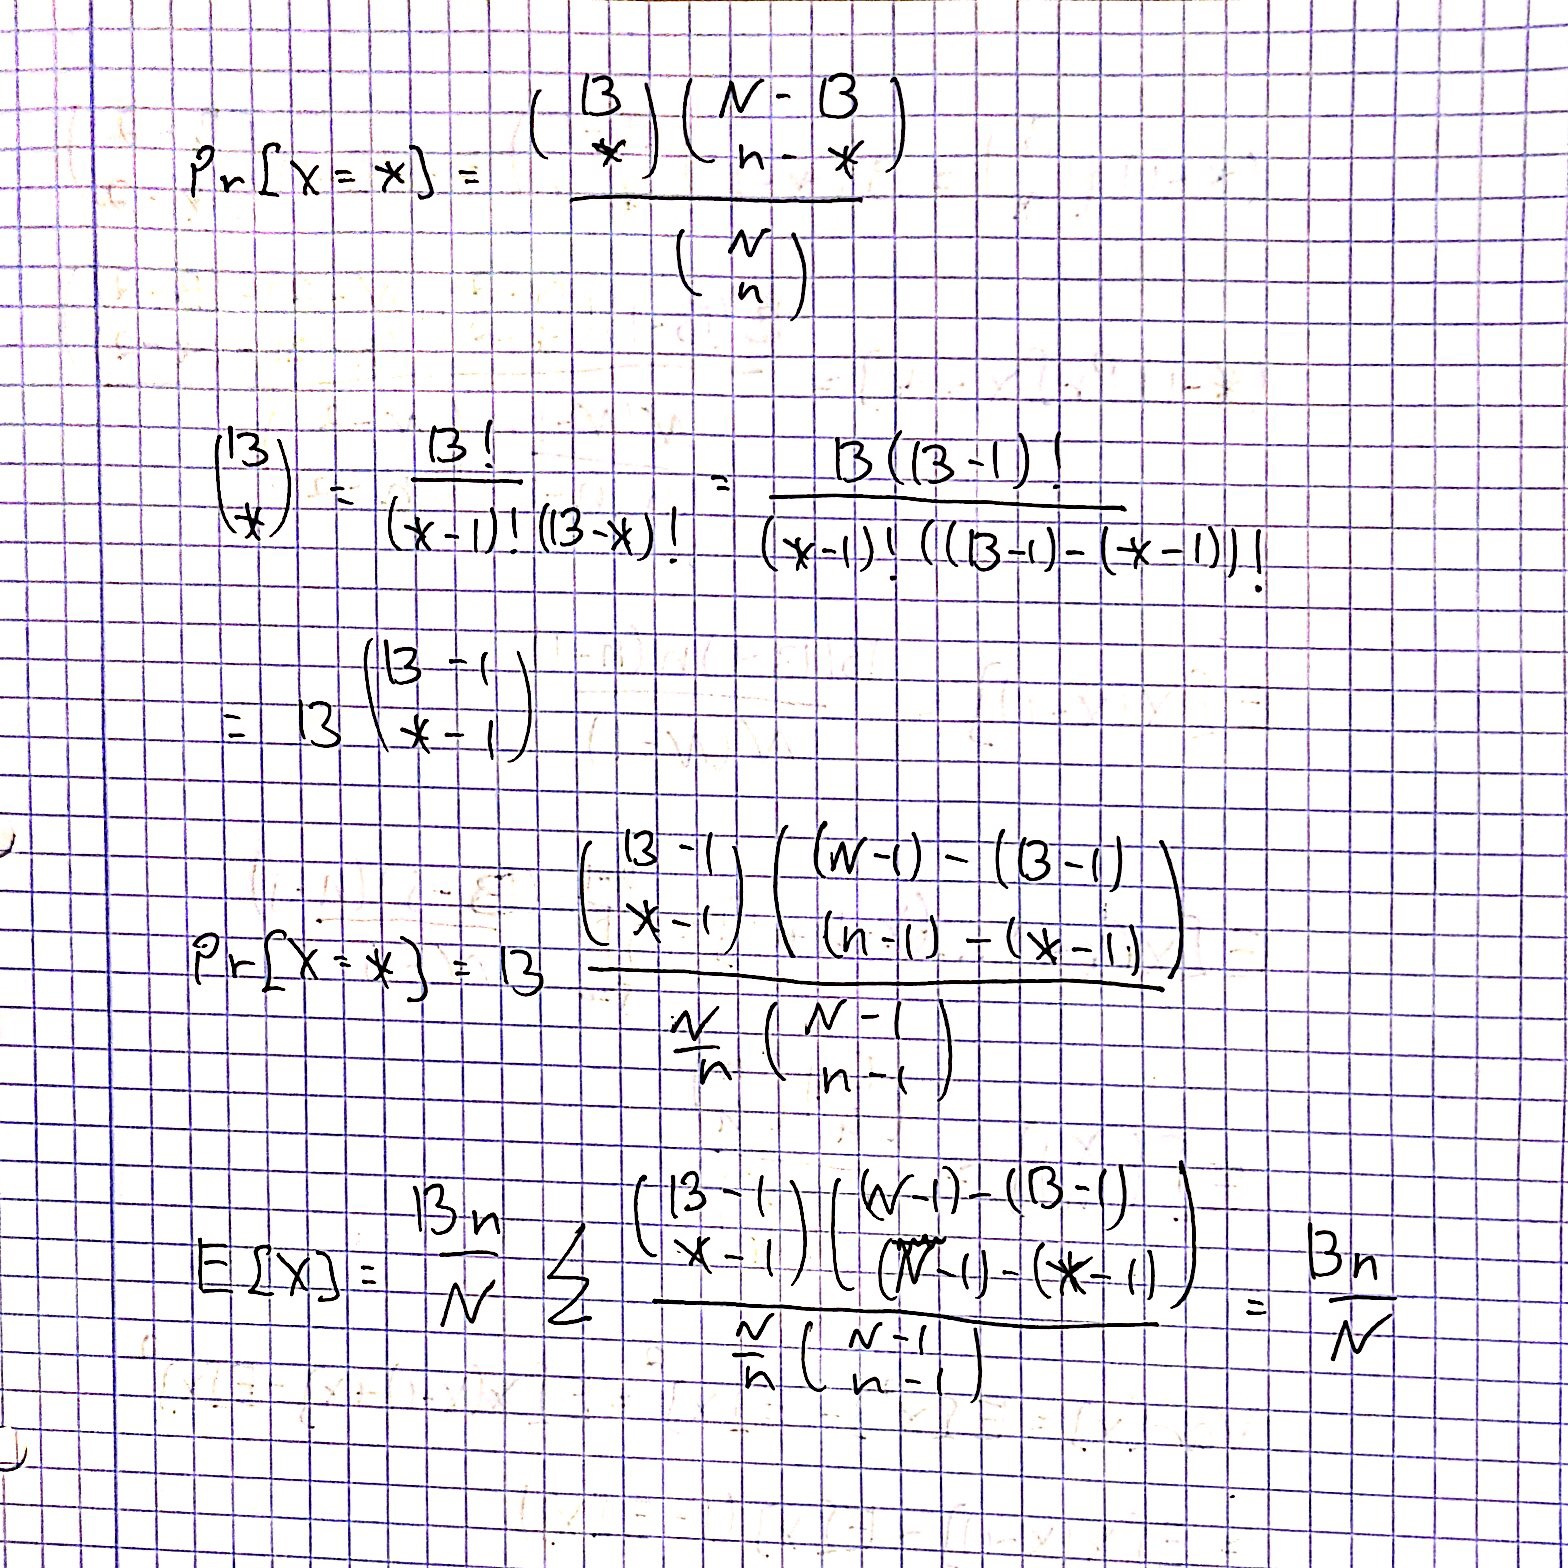
\includegraphics{3-0a.JPG} 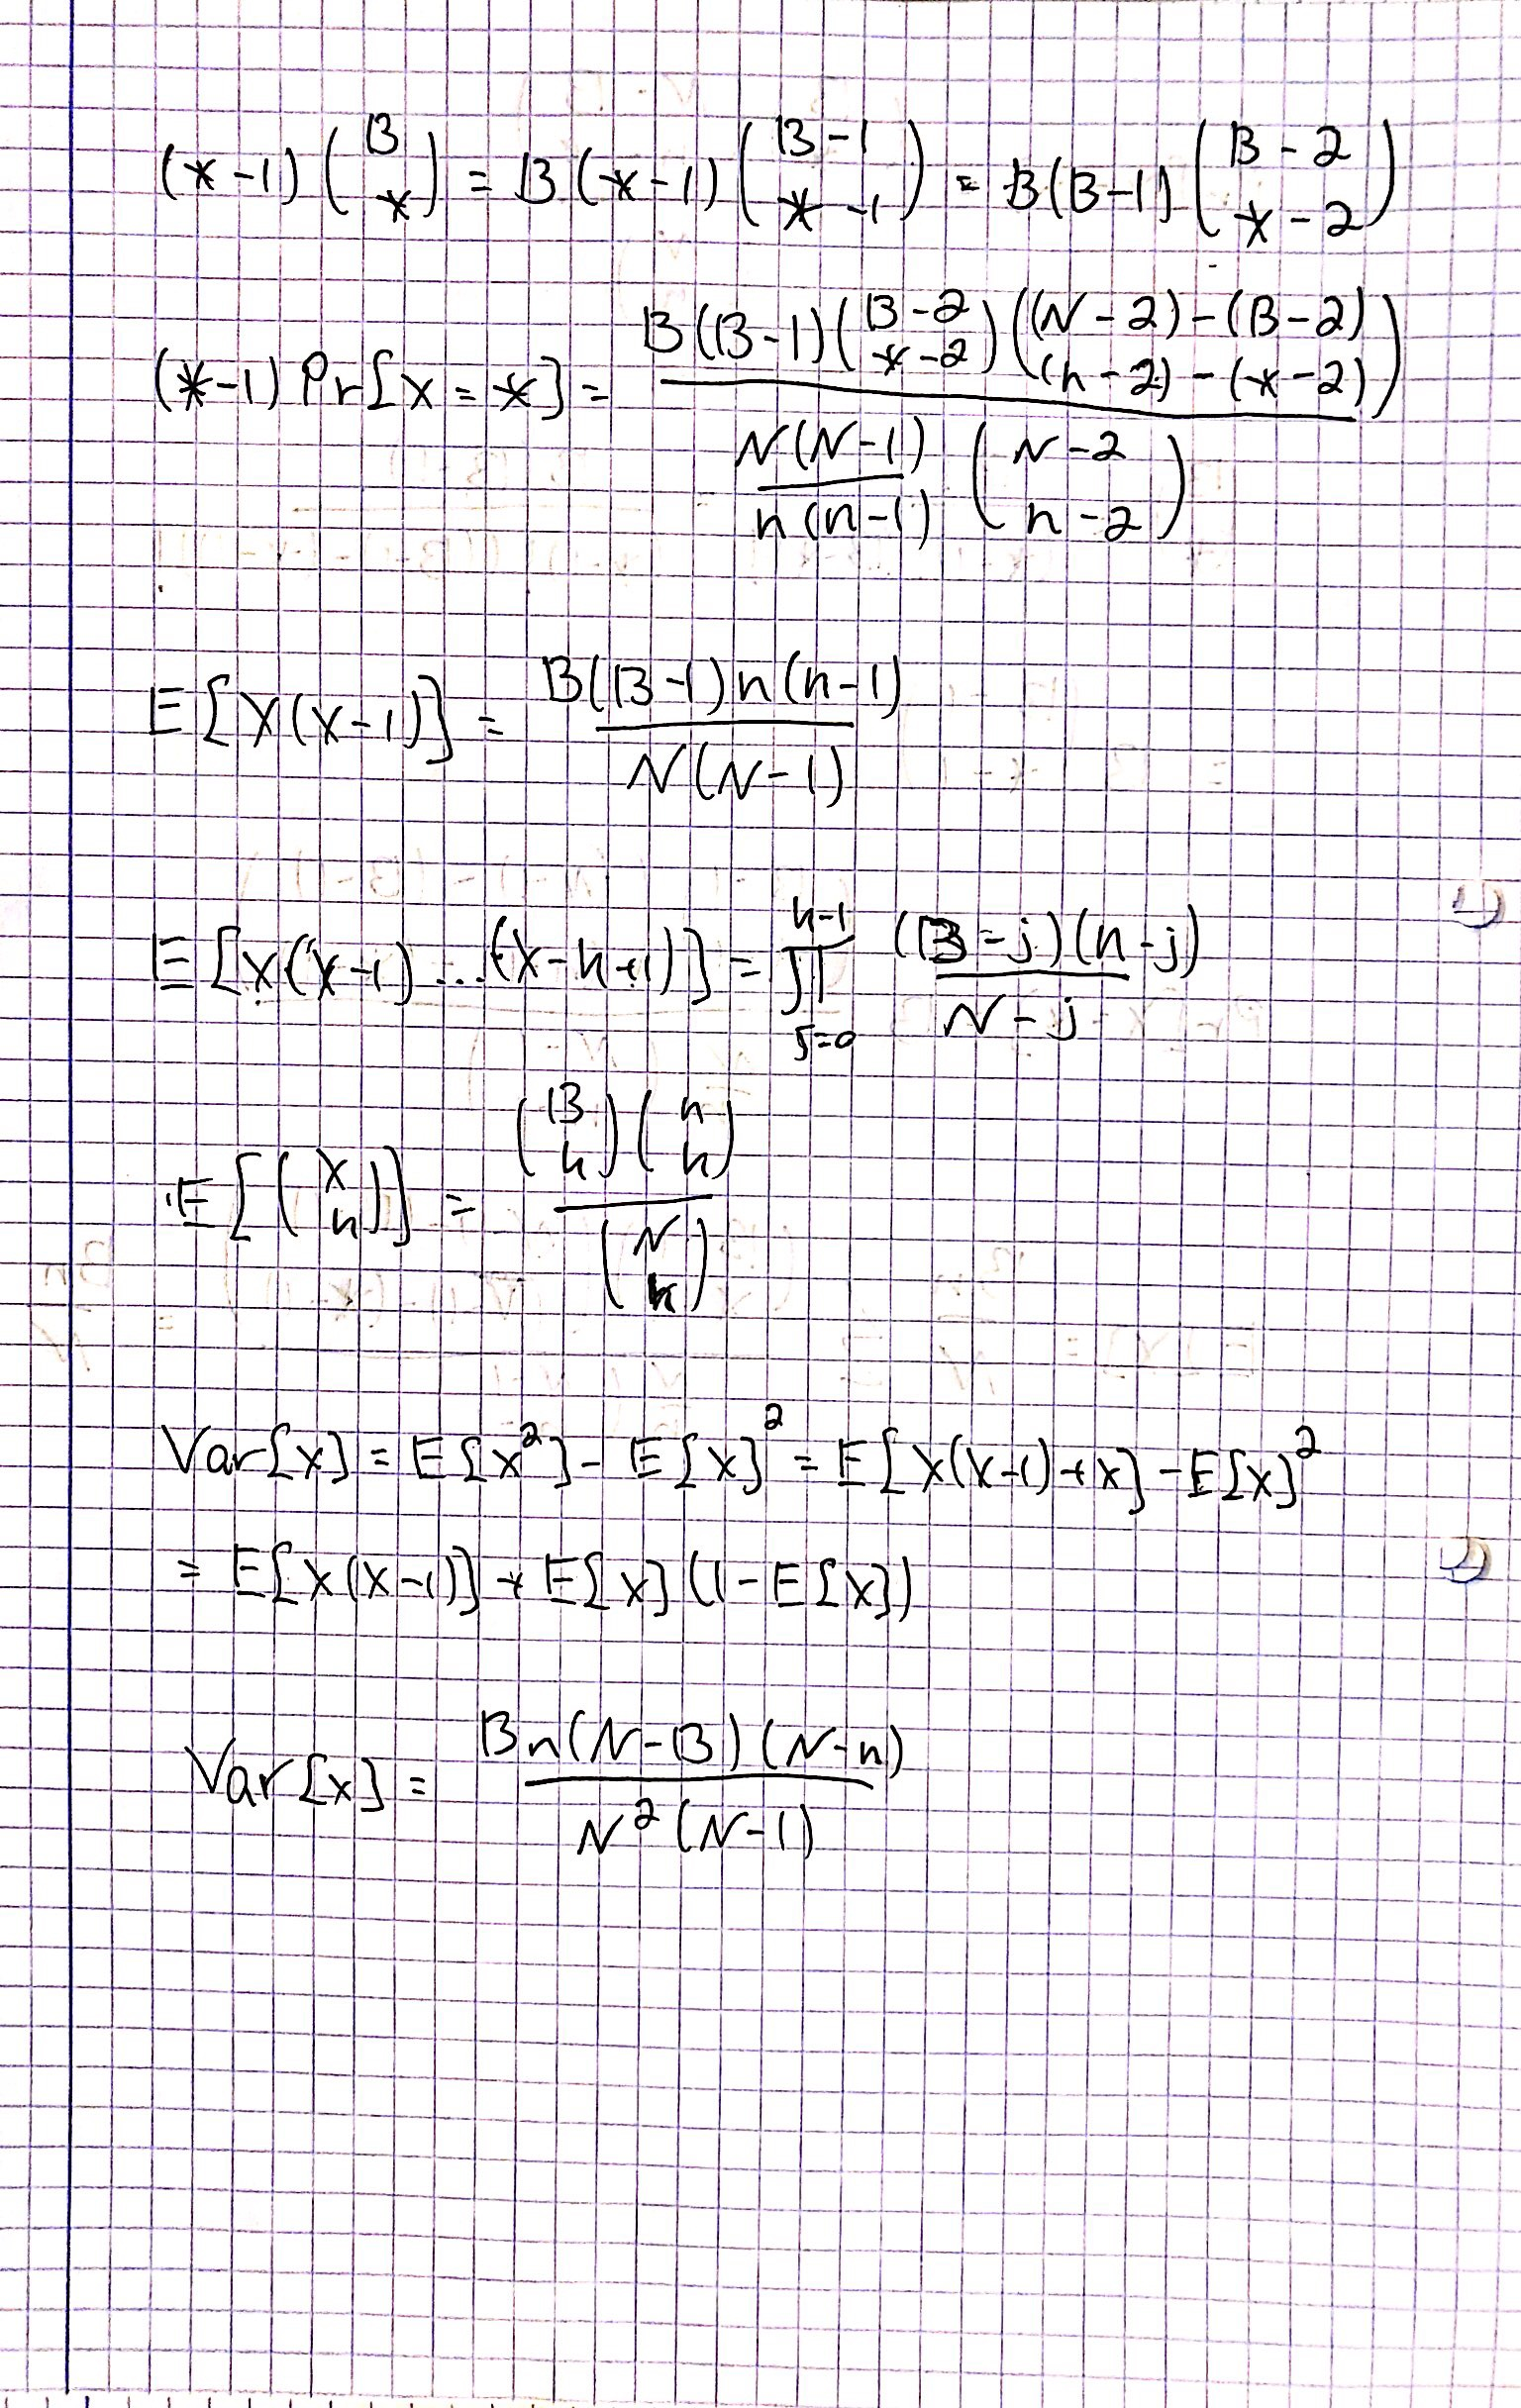
\includegraphics{3-0b.JPG}

    \hypertarget{what-is-the-probability-of-winning-b-of-winning-s}{%
\subsubsection{What is the probability of winning B? of winning
S?}\label{what-is-the-probability-of-winning-b-of-winning-s}}

    \begin{figure}
\centering
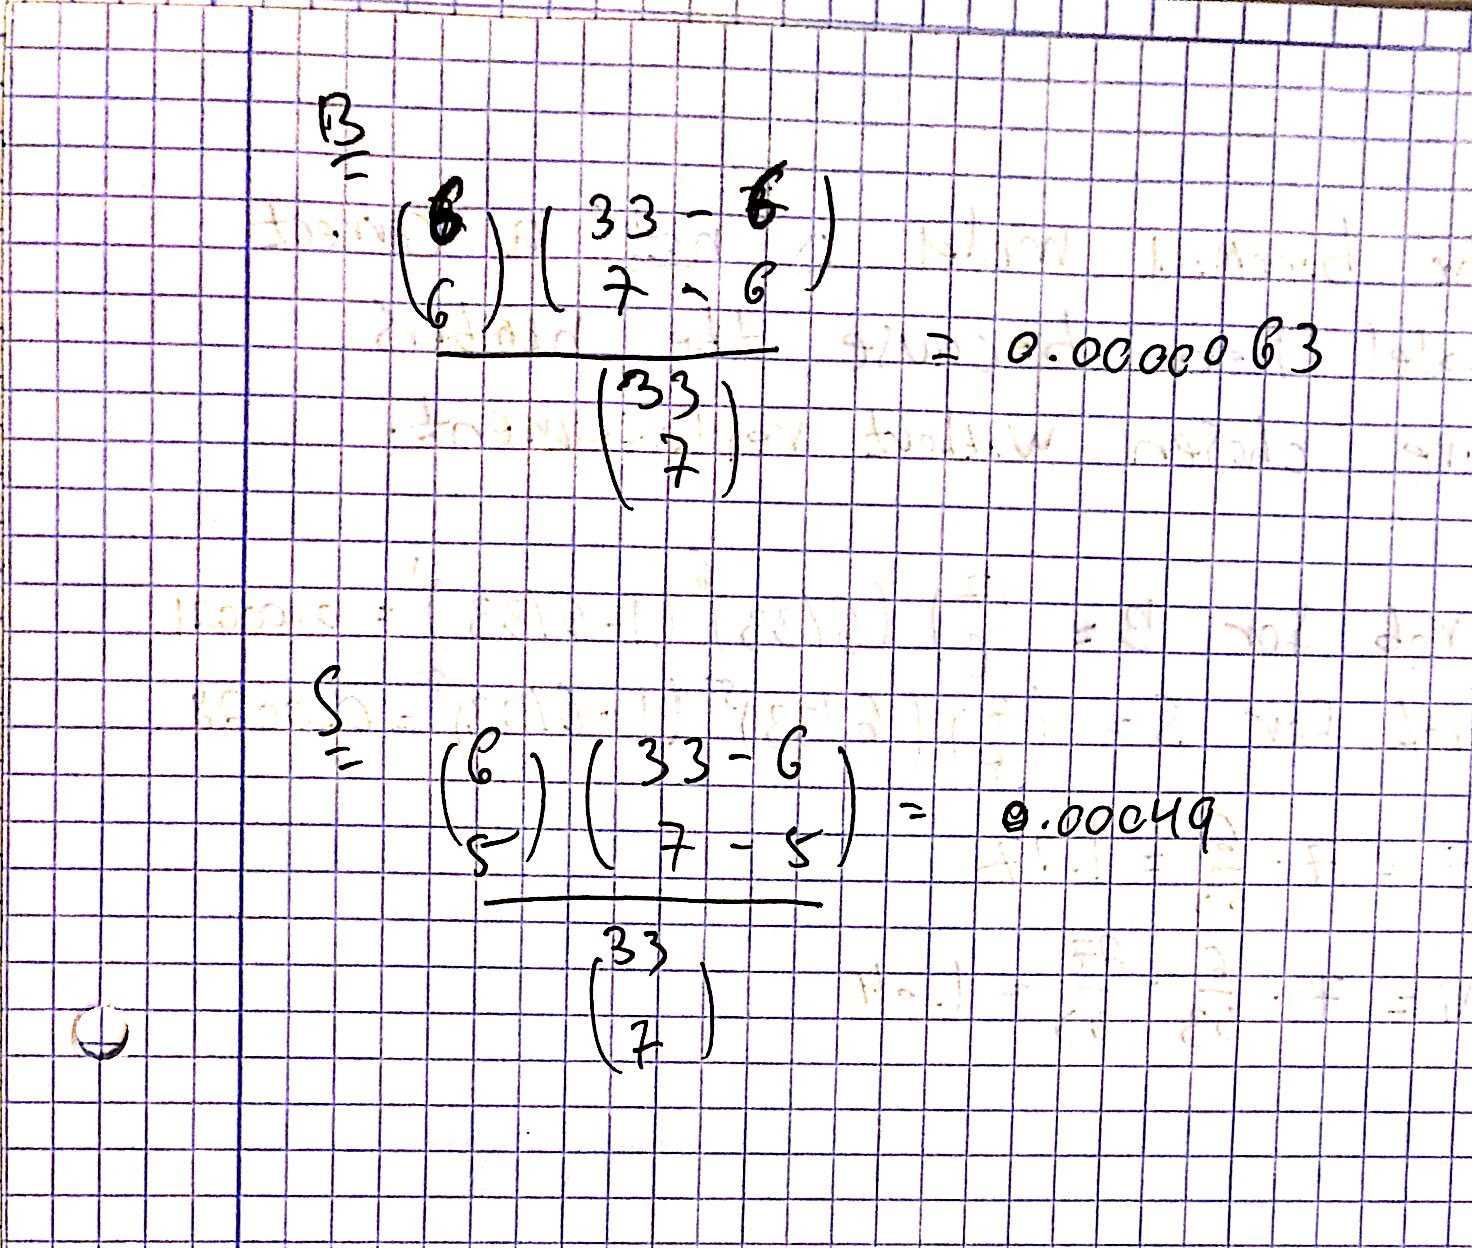
\includegraphics{3-1.JPG}
\caption{title}
\end{figure}

    \hypertarget{what-is-the-expected-gainloss-of-playing-the-randomistan-lotto-if-the-cost-of-playing-is-c}{%
\subsubsection{What is the expected gain/loss of playing the Randomistan
Lotto if the cost of playing is
C?}\label{what-is-the-expected-gainloss-of-playing-the-randomistan-lotto-if-the-cost-of-playing-is-c}}

    \begin{figure}
\centering
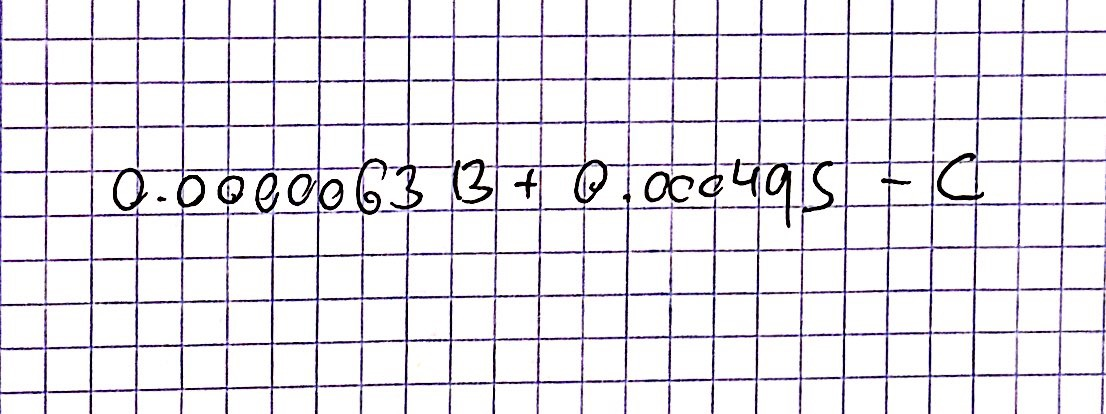
\includegraphics{3-2.JPG}
\caption{title}
\end{figure}

    \hypertarget{what-are-the-expectation-and-variance-of-the-number-of-matches-between-a-persons-selected-numbers-and-the-winning-6-numbers}{%
\subsubsection{What are the expectation and variance of the number of
matches between a person's selected numbers and the winning 6
numbers?}\label{what-are-the-expectation-and-variance-of-the-number-of-matches-between-a-persons-selected-numbers-and-the-winning-6-numbers}}

    \begin{figure}
\centering
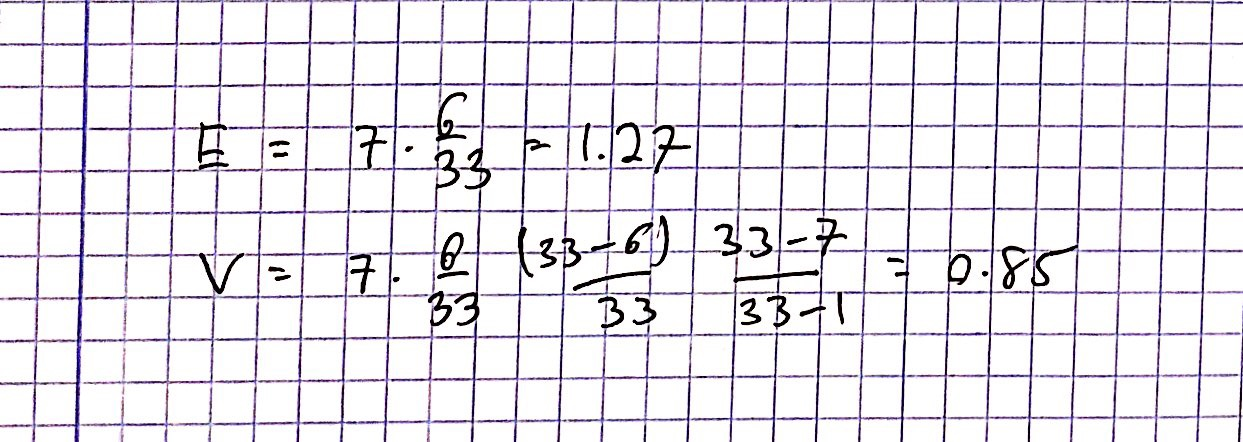
\includegraphics{3-3.JPG}
\caption{title}
\end{figure}

    \hypertarget{how-would-the-answers-to-the-previous-questions-differ-if-we-used-a-binomial-model-is-the-binomial-a-correct-model-here}{%
\subsubsection{How would the answers to the previous questions differ if
we used a binomial model? Is the binomial a correct model
here?}\label{how-would-the-answers-to-the-previous-questions-differ-if-we-used-a-binomial-model-is-the-binomial-a-correct-model-here}}

    \begin{figure}
\centering
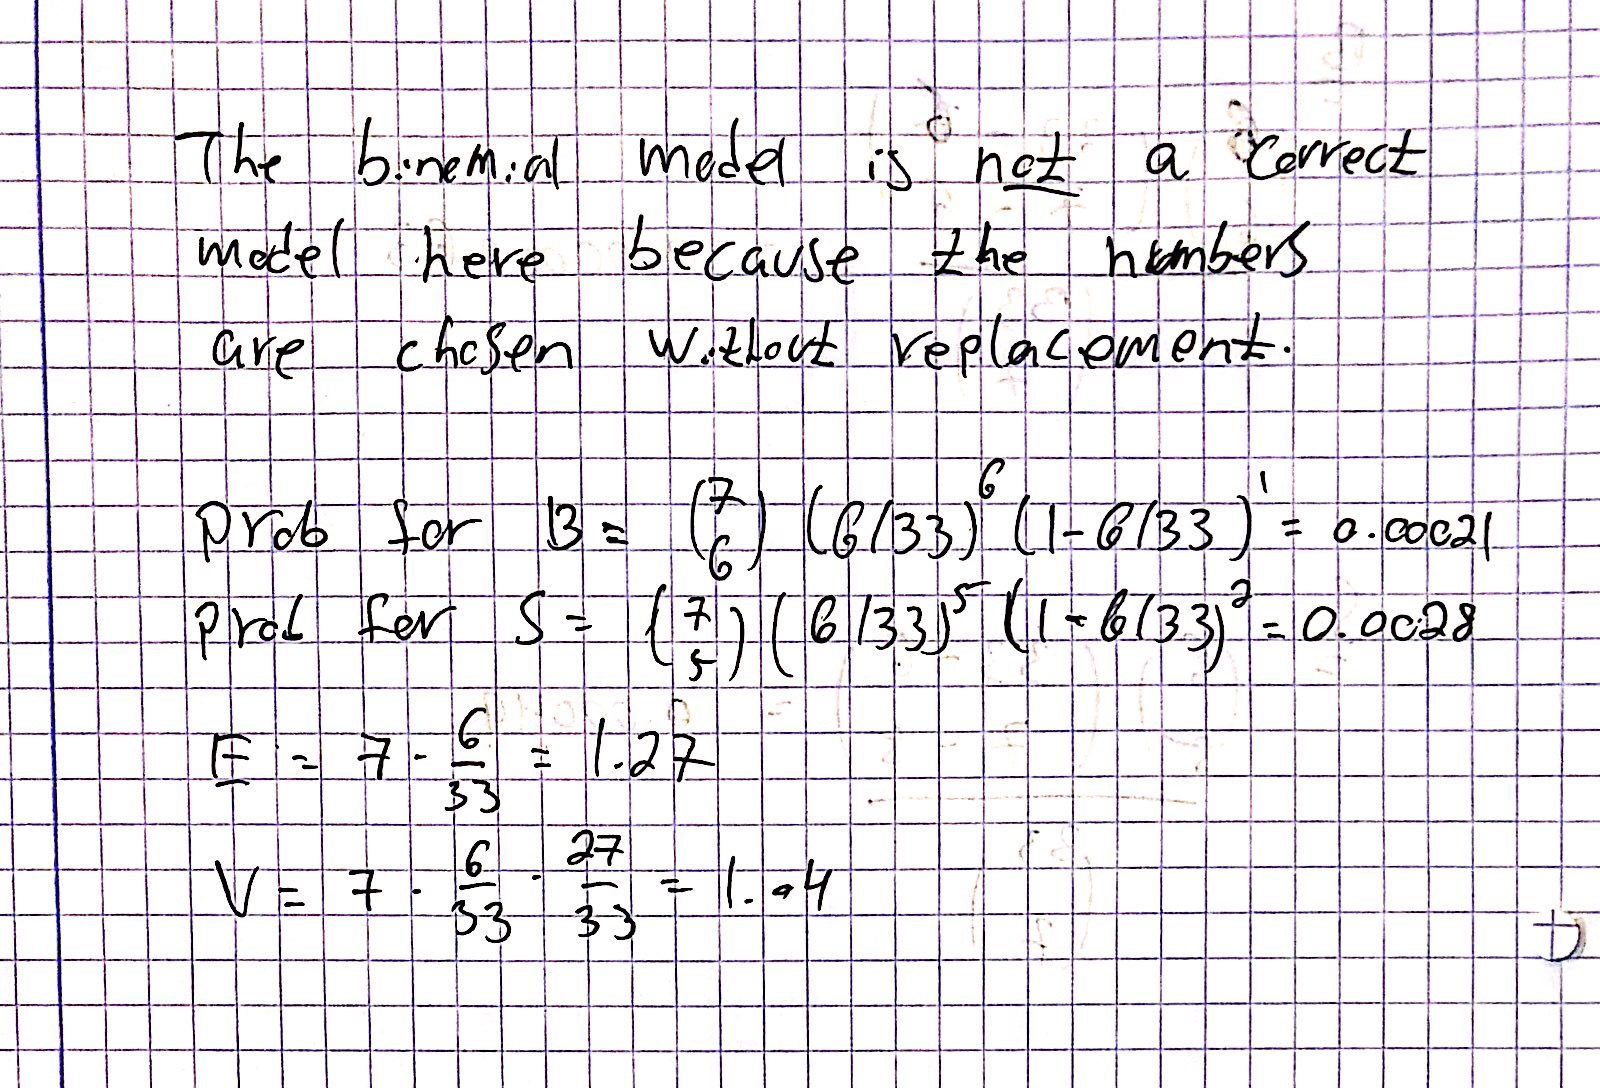
\includegraphics{3-4.JPG}
\caption{title}
\end{figure}

    \hypertarget{log-normal}{%
\section{Log Normal}\label{log-normal}}

    \hypertarget{draw-a-plot-of-the-pdfs-for-y1-and-y2-on-the-same-axes-over-the-x-range-of-0-10.}{%
\subsubsection{Draw a plot of the pdfs for Y1 and Y2 on the same axes,
over the x range of {[}0
10{]}.}\label{draw-a-plot-of-the-pdfs-for-y1-and-y2-on-the-same-axes-over-the-x-range-of-0-10.}}

    \begin{Verbatim}[commandchars=\\\{\}]
{\color{incolor}In [{\color{incolor}127}]:} \PY{k+kn}{from} \PY{n+nn}{scipy}\PY{n+nn}{.}\PY{n+nn}{stats} \PY{k}{import} \PY{n}{lognorm}\PY{p}{,} \PY{n}{norm}
          \PY{k+kn}{from} \PY{n+nn}{numpy}\PY{n+nn}{.}\PY{n+nn}{core} \PY{k}{import} \PY{n}{exp}
          \PY{k+kn}{import} \PY{n+nn}{numpy} \PY{k}{as} \PY{n+nn}{np}
          \PY{k+kn}{import} \PY{n+nn}{matplotlib}\PY{n+nn}{.}\PY{n+nn}{pyplot} \PY{k}{as} \PY{n+nn}{plt}
          
          \PY{n}{distX} \PY{o}{=} \PY{n}{lognorm}\PY{p}{(}\PY{n}{s}\PY{o}{=}\PY{l+m+mf}{0.25}\PY{p}{,} \PY{n}{scale}\PY{o}{=}\PY{n}{exp}\PY{p}{(}\PY{l+m+mi}{0}\PY{p}{)}\PY{p}{)}
          \PY{n}{distY} \PY{o}{=} \PY{n}{lognorm}\PY{p}{(}\PY{n}{s}\PY{o}{=}\PY{l+m+mi}{1}\PY{p}{,} \PY{n}{scale}\PY{o}{=}\PY{n}{exp}\PY{p}{(}\PY{l+m+mi}{0}\PY{p}{)}\PY{p}{)}
          
          \PY{n}{x} \PY{o}{=} \PY{n}{np}\PY{o}{.}\PY{n}{linspace}\PY{p}{(}\PY{l+m+mi}{0}\PY{p}{,} \PY{l+m+mi}{10}\PY{p}{,} \PY{l+m+mi}{200}\PY{p}{)}
          \PY{n}{pdfX} \PY{o}{=} \PY{n}{distX}\PY{o}{.}\PY{n}{pdf}\PY{p}{(}\PY{n}{x}\PY{p}{)}
          \PY{n}{pdfY} \PY{o}{=} \PY{n}{distY}\PY{o}{.}\PY{n}{pdf}\PY{p}{(}\PY{n}{x}\PY{p}{)}
          \PY{n}{plt}\PY{o}{.}\PY{n}{plot}\PY{p}{(}\PY{n}{x}\PY{p}{,} \PY{n}{pdfX}\PY{p}{,} \PY{n}{label}\PY{o}{=}\PY{l+s+s1}{\PYZsq{}}\PY{l+s+s1}{Y1}\PY{l+s+s1}{\PYZsq{}}\PY{p}{)}
          \PY{n}{plt}\PY{o}{.}\PY{n}{plot}\PY{p}{(}\PY{n}{x}\PY{p}{,} \PY{n}{pdfY}\PY{p}{,} \PY{n}{label}\PY{o}{=}\PY{l+s+s1}{\PYZsq{}}\PY{l+s+s1}{Y2}\PY{l+s+s1}{\PYZsq{}}\PY{p}{)}
          \PY{n}{plt}\PY{o}{.}\PY{n}{xlabel}\PY{p}{(}\PY{l+s+s1}{\PYZsq{}}\PY{l+s+s1}{x}\PY{l+s+s1}{\PYZsq{}}\PY{p}{)}
          \PY{n}{plt}\PY{o}{.}\PY{n}{ylabel}\PY{p}{(}\PY{l+s+s1}{\PYZsq{}}\PY{l+s+s1}{pdf(x)}\PY{l+s+s1}{\PYZsq{}}\PY{p}{)}
          \PY{n}{plt}\PY{o}{.}\PY{n}{legend}\PY{p}{(}\PY{p}{)}
          
          \PY{n}{plt}\PY{o}{.}\PY{n}{title}\PY{p}{(}\PY{l+s+sa}{r}\PY{l+s+s1}{\PYZsq{}}\PY{l+s+s1}{pdf of \PYZdl{}Y1}\PY{l+s+s1}{\PYZbs{}}\PY{l+s+s1}{sim}\PY{l+s+s1}{\PYZbs{}}\PY{l+s+s1}{mathrm}\PY{l+s+si}{\PYZob{}LogNormal\PYZcb{}}\PY{l+s+s1}{(0,0.25)\PYZdl{} and \PYZdl{}Y2}\PY{l+s+s1}{\PYZbs{}}\PY{l+s+s1}{sim}\PY{l+s+s1}{\PYZbs{}}\PY{l+s+s1}{mathrm}\PY{l+s+si}{\PYZob{}LogNormal\PYZcb{}}\PY{l+s+s1}{(0,1)\PYZdl{}}\PY{l+s+s1}{\PYZsq{}}\PY{p}{)}
          \PY{n}{plt}\PY{o}{.}\PY{n}{show}\PY{p}{(}\PY{p}{)}
\end{Verbatim}


    \begin{center}
    \adjustimage{max size={0.9\linewidth}{0.9\paperheight}}{output_41_0.png}
    \end{center}
    { \hspace*{\fill} \\}
    
    \hypertarget{what-is-ey1-ey2}{%
\subsubsection{What is E(Y1)? E(Y2)?}\label{what-is-ey1-ey2}}

    \begin{Verbatim}[commandchars=\\\{\}]
{\color{incolor}In [{\color{incolor}132}]:} \PY{n+nb}{print} \PY{p}{(}\PY{l+s+s1}{\PYZsq{}}\PY{l+s+s1}{E[Y] = exp(μ + (σ\PYZca{}2)/2)}\PY{l+s+s1}{\PYZsq{}}\PY{p}{)}
          \PY{n+nb}{print} \PY{p}{(}\PY{l+s+s1}{\PYZsq{}}\PY{l+s+s1}{E[Y1] = }\PY{l+s+si}{\PYZpc{}s}\PY{l+s+s1}{\PYZsq{}} \PY{o}{\PYZpc{}} \PY{n}{exp}\PY{p}{(}\PY{l+m+mi}{0} \PY{o}{+} \PY{p}{(}\PY{l+m+mf}{0.25} \PY{o}{*}\PY{o}{*} \PY{l+m+mi}{2}\PY{p}{)} \PY{o}{/} \PY{l+m+mi}{2}\PY{p}{)}\PY{p}{)}
          \PY{n+nb}{print} \PY{p}{(}\PY{l+s+s1}{\PYZsq{}}\PY{l+s+s1}{E[Y2] = }\PY{l+s+si}{\PYZpc{}s}\PY{l+s+s1}{\PYZsq{}} \PY{o}{\PYZpc{}} \PY{n}{exp}\PY{p}{(}\PY{l+m+mi}{0} \PY{o}{+} \PY{p}{(}\PY{l+m+mi}{1} \PY{o}{*}\PY{o}{*} \PY{l+m+mi}{2}\PY{p}{)} \PY{o}{/} \PY{l+m+mi}{2}\PY{p}{)}\PY{p}{)}
\end{Verbatim}


    \begin{Verbatim}[commandchars=\\\{\}]
E[Y] = exp(μ + (σ\^{}2)/2)
E[Y1] = 1.0317434075
E[Y2] = 1.6487212707

    \end{Verbatim}

    \hypertarget{what-is-the-probability-of-y1-being-more-than-4-stds-larger-than-its-mean}{%
\subsubsection{What is the probability of Y1 being more than 4 stds
larger than its
mean?}\label{what-is-the-probability-of-y1-being-more-than-4-stds-larger-than-its-mean}}

    \begin{figure}
\centering
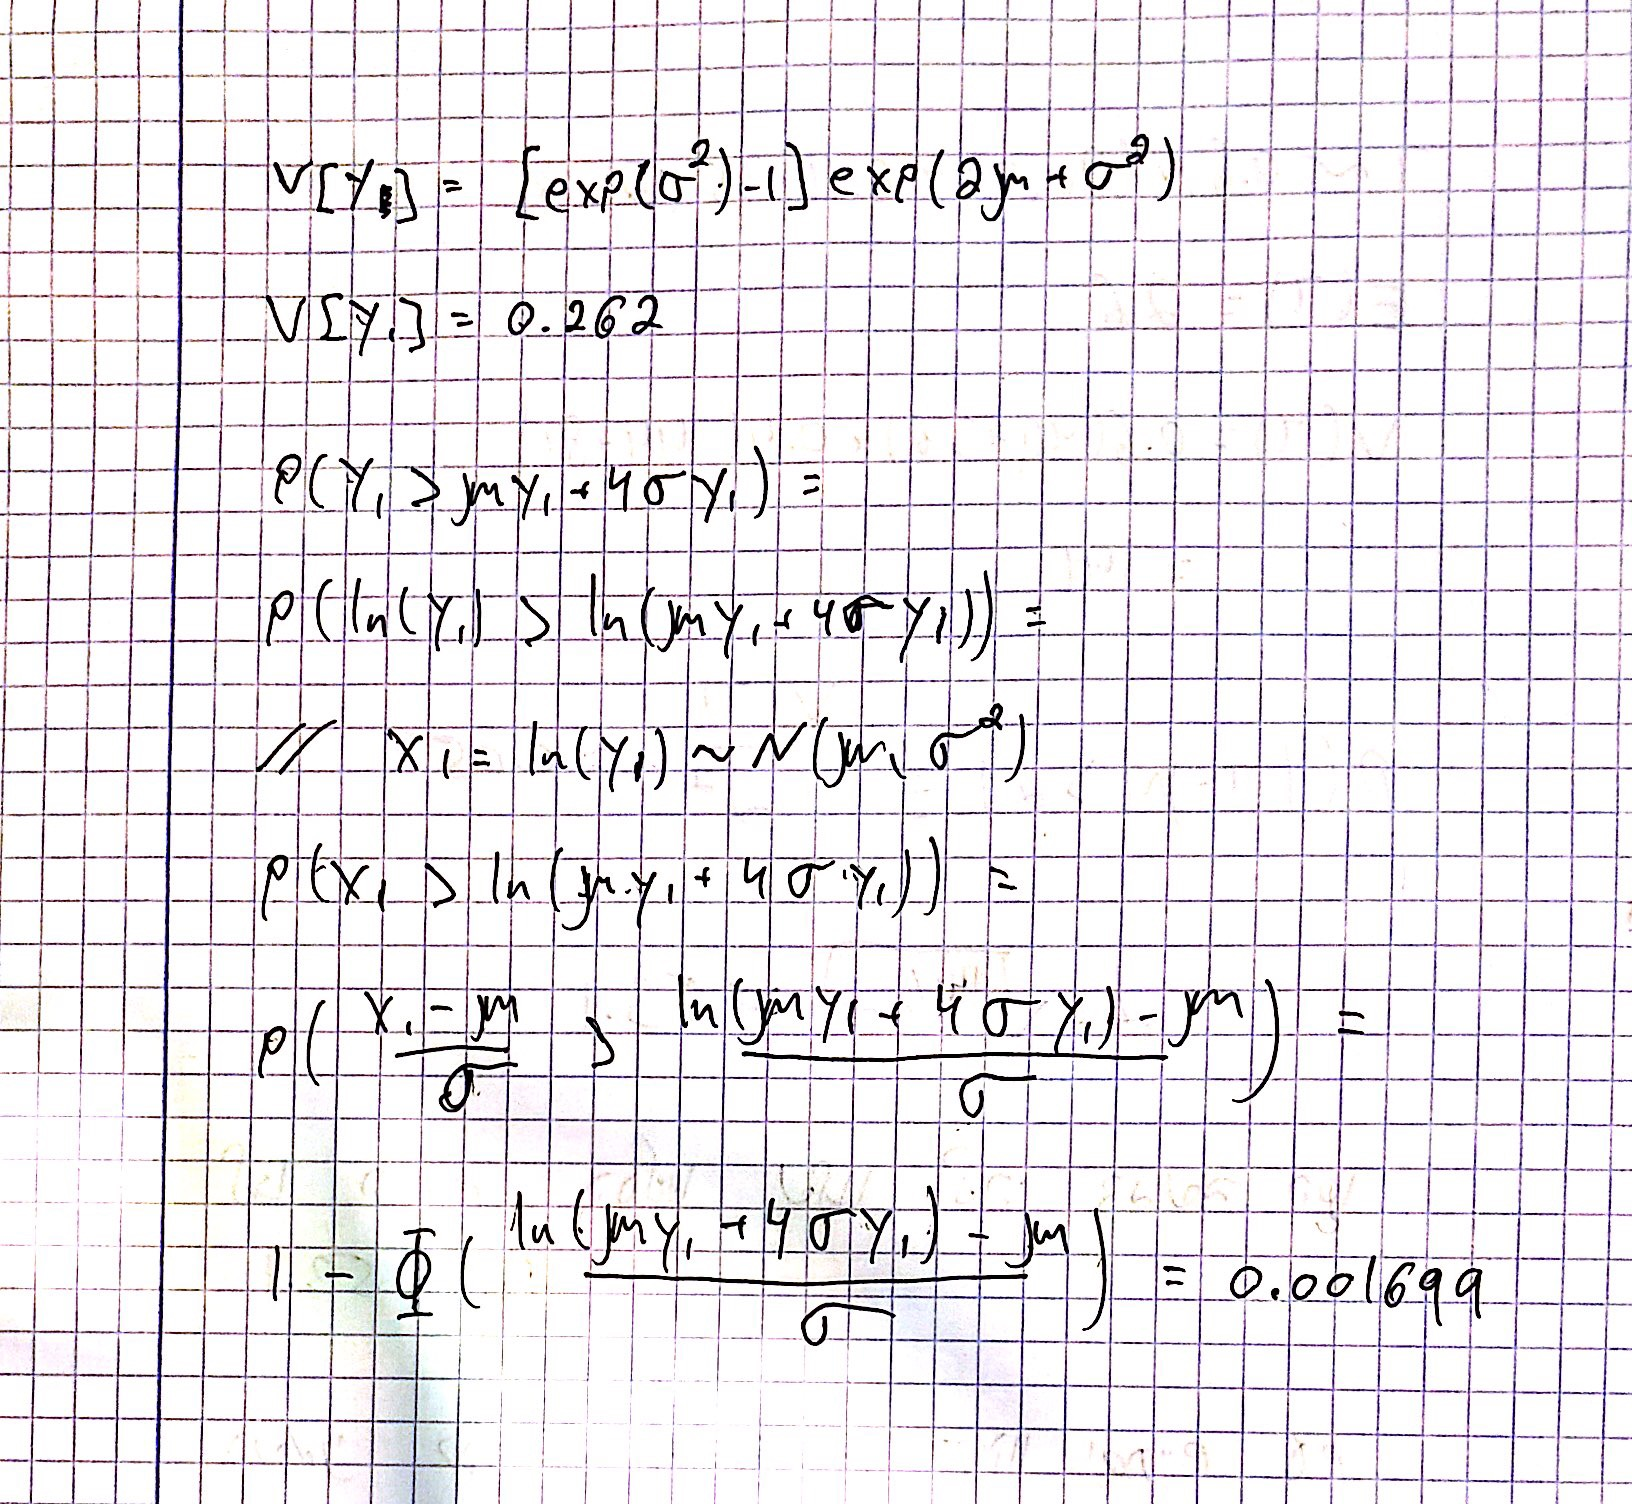
\includegraphics{4-3.JPG}
\caption{title}
\end{figure}

    \hypertarget{what-is-the-probability-of-y2-being-more-than-4-stds-larger-than-its-mean}{%
\subsubsection{What is the probability of Y2 being more than 4 stds
larger than its
mean?}\label{what-is-the-probability-of-y2-being-more-than-4-stds-larger-than-its-mean}}

    \begin{figure}
\centering
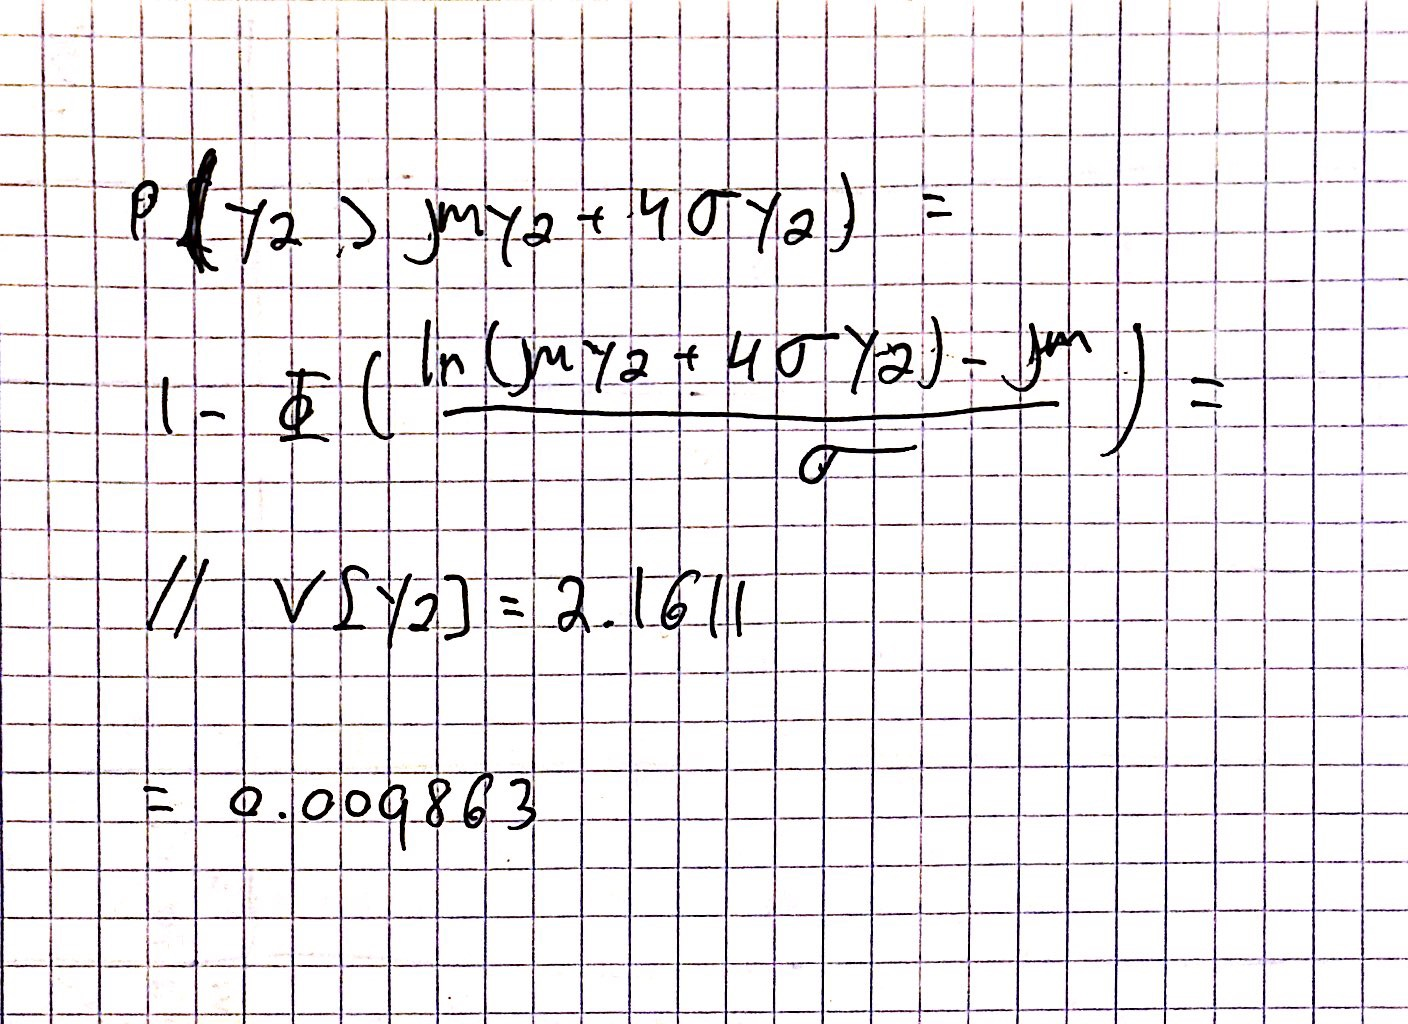
\includegraphics{4-4.JPG}
\caption{title}
\end{figure}

    \hypertarget{what-is-the-iqr-of-y1-of-y2}{%
\subsubsection{What is the IQR of Y1? Of
Y2?}\label{what-is-the-iqr-of-y1-of-y2}}

    \begin{figure}
\centering
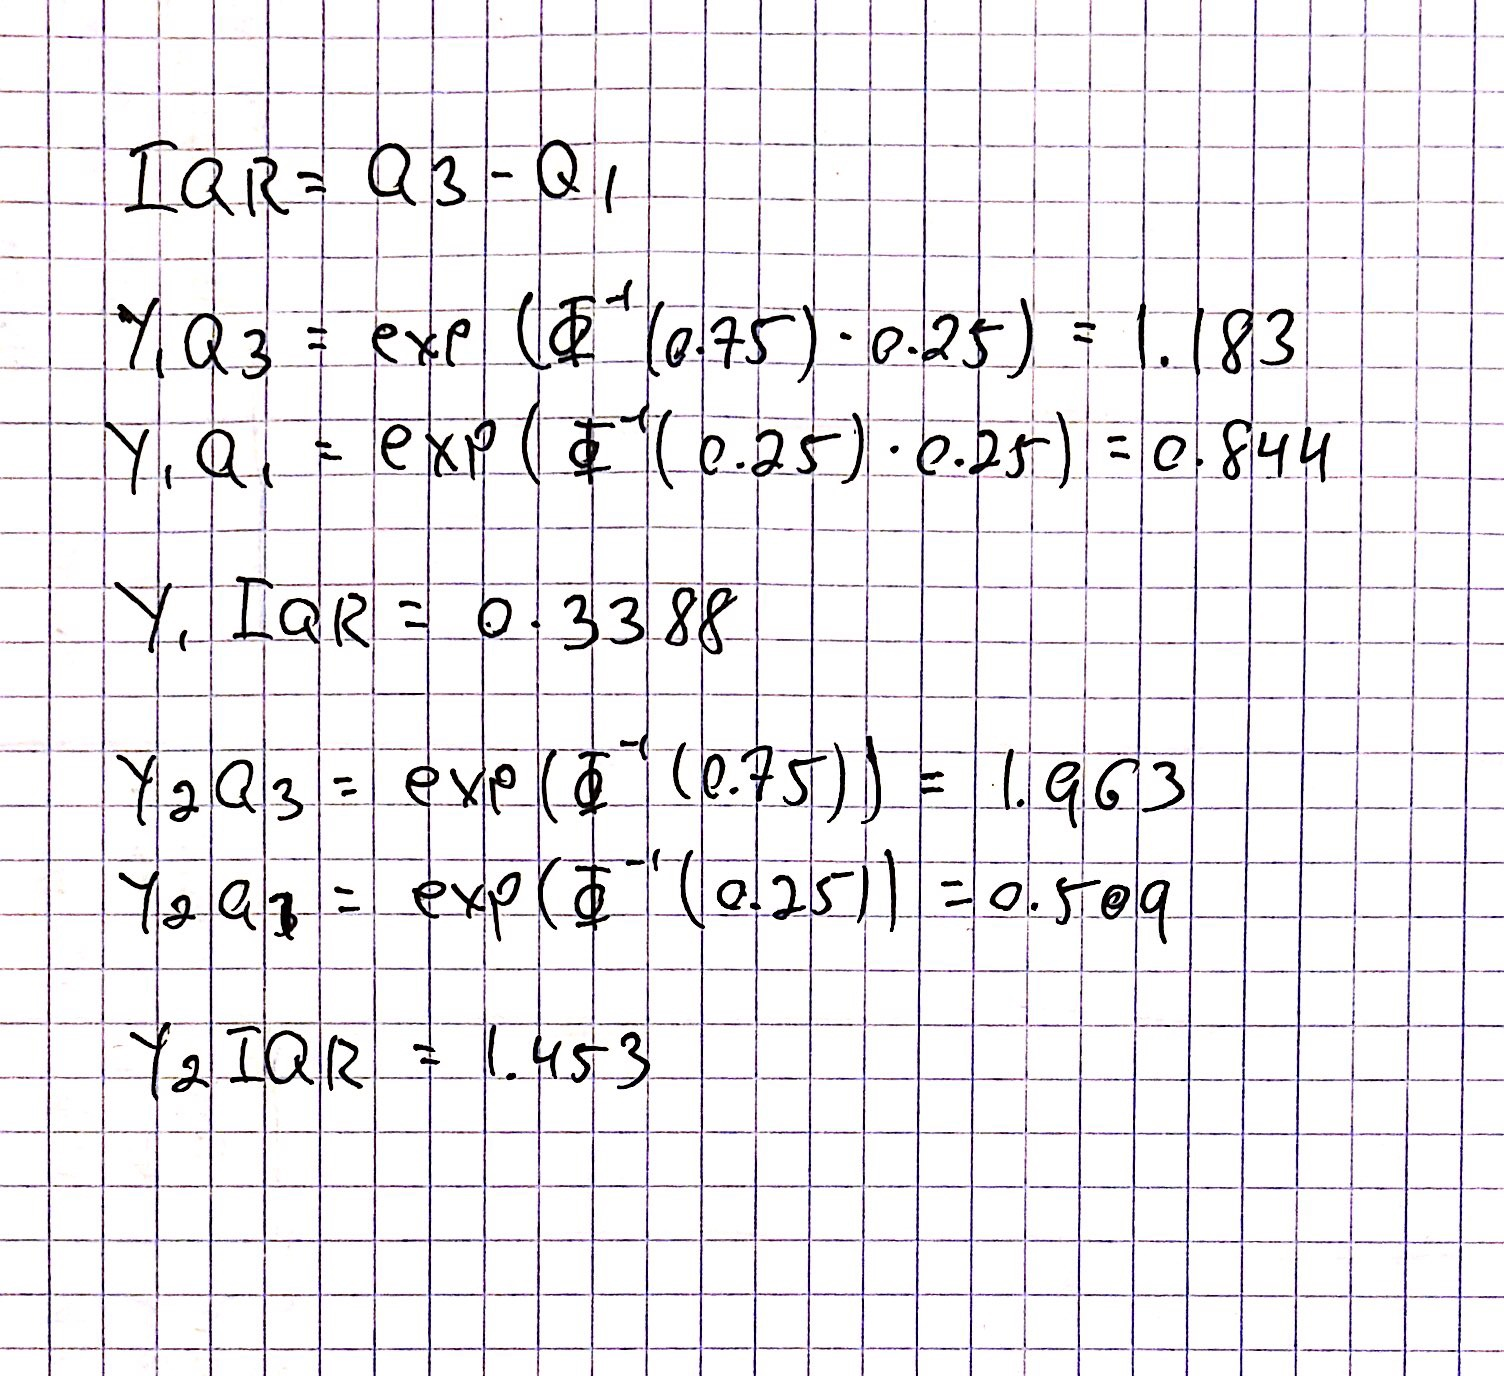
\includegraphics{4-5.JPG}
\caption{title}
\end{figure}

    \hypertarget{clt-for-markov-chains}{%
\section{CLT for Markov chains}\label{clt-for-markov-chains}}

    \hypertarget{construct-1000-trajectories-each-of-length-20.}{%
\subsubsection{Construct 1000 trajectories, each of length
20.}\label{construct-1000-trajectories-each-of-length-20.}}

    \begin{Verbatim}[commandchars=\\\{\}]
{\color{incolor}In [{\color{incolor}193}]:} \PY{k+kn}{import} \PY{n+nn}{random}
          \PY{k+kn}{import} \PY{n+nn}{numpy} \PY{k}{as} \PY{n+nn}{np}
          
          \PY{n}{transition\PYZus{}matrix} \PY{o}{=} \PY{p}{[}
              \PY{p}{[}\PY{l+m+mf}{0.5}\PY{p}{,}  \PY{l+m+mf}{0.25}\PY{p}{,} \PY{l+m+mi}{0}\PY{p}{,}    \PY{l+m+mi}{0}\PY{p}{,}    \PY{l+m+mi}{0}\PY{p}{,}    \PY{l+m+mf}{0.25}\PY{p}{]}\PY{p}{,}
              \PY{p}{[}\PY{l+m+mf}{0.25}\PY{p}{,} \PY{l+m+mf}{0.5}\PY{p}{,}  \PY{l+m+mf}{0.25}\PY{p}{,} \PY{l+m+mi}{0}\PY{p}{,}    \PY{l+m+mi}{0}\PY{p}{,}    \PY{l+m+mi}{0}\PY{p}{]}\PY{p}{,}
              \PY{p}{[}\PY{l+m+mi}{0}\PY{p}{,}    \PY{l+m+mf}{0.25}\PY{p}{,} \PY{l+m+mf}{0.5}\PY{p}{,}  \PY{l+m+mf}{0.25}\PY{p}{,} \PY{l+m+mi}{0}\PY{p}{,}    \PY{l+m+mi}{0}\PY{p}{]}\PY{p}{,}
              \PY{p}{[}\PY{l+m+mi}{0}\PY{p}{,}    \PY{l+m+mi}{0}\PY{p}{,}    \PY{l+m+mf}{0.25}\PY{p}{,} \PY{l+m+mf}{0.5}\PY{p}{,}  \PY{l+m+mf}{0.25}\PY{p}{,} \PY{l+m+mi}{0}\PY{p}{]}\PY{p}{,}
              \PY{p}{[}\PY{l+m+mi}{0}\PY{p}{,}    \PY{l+m+mi}{0}\PY{p}{,}    \PY{l+m+mi}{0}\PY{p}{,}    \PY{l+m+mf}{0.25}\PY{p}{,} \PY{l+m+mf}{0.5}\PY{p}{,}  \PY{l+m+mf}{0.25}\PY{p}{]}\PY{p}{,}
              \PY{p}{[}\PY{l+m+mf}{0.25}\PY{p}{,} \PY{l+m+mi}{0}\PY{p}{,}    \PY{l+m+mi}{0}\PY{p}{,}    \PY{l+m+mi}{0}\PY{p}{,}    \PY{l+m+mf}{0.25}\PY{p}{,} \PY{l+m+mf}{0.5}\PY{p}{]}
          \PY{p}{]}
          
          \PY{k}{def} \PY{n+nf}{create\PYZus{}trajectories}\PY{p}{(}\PY{n}{n}\PY{p}{)}\PY{p}{:}
              \PY{n}{trajectories} \PY{o}{=} \PY{p}{[}\PY{p}{]}
              \PY{k}{for} \PY{n}{i} \PY{o+ow}{in} \PY{n+nb}{range}\PY{p}{(}\PY{l+m+mi}{0}\PY{p}{,} \PY{l+m+mi}{1000}\PY{p}{)}\PY{p}{:}
                  \PY{n}{first\PYZus{}roll} \PY{o}{=} \PY{n}{random}\PY{o}{.}\PY{n}{randint}\PY{p}{(}\PY{l+m+mi}{1}\PY{p}{,} \PY{l+m+mi}{6}\PY{p}{)}
                  \PY{n}{rolls} \PY{o}{=} \PY{p}{[}\PY{n}{first\PYZus{}roll}\PY{p}{]}
          
                  \PY{k}{for} \PY{n}{i} \PY{o+ow}{in} \PY{n+nb}{range}\PY{p}{(}\PY{l+m+mi}{0}\PY{p}{,} \PY{n}{n}\PY{o}{\PYZhy{}}\PY{l+m+mi}{1}\PY{p}{)}\PY{p}{:}
                      \PY{n}{xi} \PY{o}{=} \PY{n}{np}\PY{o}{.}\PY{n}{random}\PY{o}{.}\PY{n}{choice}\PY{p}{(}\PY{p}{[}\PY{l+m+mi}{1}\PY{p}{,} \PY{l+m+mi}{2}\PY{p}{,} \PY{l+m+mi}{3}\PY{p}{,} \PY{l+m+mi}{4}\PY{p}{,} \PY{l+m+mi}{5}\PY{p}{,} \PY{l+m+mi}{6}\PY{p}{]}\PY{p}{,} \PY{n}{p}\PY{o}{=}\PY{n}{transition\PYZus{}matrix}\PY{p}{[}\PY{n}{rolls}\PY{p}{[}\PY{n}{i}\PY{p}{]} \PY{o}{\PYZhy{}} \PY{l+m+mi}{1}\PY{p}{]}\PY{p}{)}
                      \PY{n}{rolls}\PY{o}{.}\PY{n}{append}\PY{p}{(}\PY{n}{xi}\PY{p}{)}
          
                  \PY{n}{trajectories}\PY{o}{.}\PY{n}{append}\PY{p}{(}\PY{n}{rolls}\PY{p}{)}
              \PY{k}{return} \PY{n}{trajectories}
          
          \PY{n}{trajectories\PYZus{}20} \PY{o}{=} \PY{n}{create\PYZus{}trajectories}\PY{p}{(}\PY{l+m+mi}{20}\PY{p}{)}
\end{Verbatim}


    \hypertarget{what-do-you-expect-the-average-value-of-all-20-numbers-in-a-trajectory-to-be}{%
\paragraph{What do you expect the average value of all 20 numbers in a
trajectory to
be?}\label{what-do-you-expect-the-average-value-of-all-20-numbers-in-a-trajectory-to-be}}

The main diaigonal has the largest probabilty which means that it if the
i roll was n the i+1 roll will probably also be n. Therefore the first
roll is very important. However because the sum of probabilities of each
dice side is equal (=1) I expect the average to be 3.5.

    \hypertarget{compute-the-average-value-of-each-such-trajectory.-draw-a-histogram-of-the-1000-numbers-you-received-using-100-bins.}{%
\paragraph{Compute the average value of each such trajectory. Draw a
histogram of the 1000 numbers you received, using 100
bins.}\label{compute-the-average-value-of-each-such-trajectory.-draw-a-histogram-of-the-1000-numbers-you-received-using-100-bins.}}

    \begin{Verbatim}[commandchars=\\\{\}]
{\color{incolor}In [{\color{incolor}203}]:} \PY{k+kn}{from} \PY{n+nn}{matplotlib} \PY{k}{import} \PY{n}{pyplot} \PY{k}{as} \PY{n}{plt}
          \PY{k+kn}{import} \PY{n+nn}{math}
          
          \PY{k}{def} \PY{n+nf}{calc\PYZus{}avg}\PY{p}{(}\PY{n}{trajectories}\PY{p}{)}\PY{p}{:}
              \PY{n}{avg} \PY{o}{=} \PY{p}{[}\PY{p}{]}
              \PY{k}{for} \PY{n}{i} \PY{o+ow}{in} \PY{n+nb}{range}\PY{p}{(}\PY{l+m+mi}{0}\PY{p}{,} \PY{l+m+mi}{1000}\PY{p}{)}\PY{p}{:}
                  \PY{n}{avg}\PY{o}{.}\PY{n}{append}\PY{p}{(}\PY{n}{np}\PY{o}{.}\PY{n}{average}\PY{p}{(}\PY{n}{np}\PY{o}{.}\PY{n}{array}\PY{p}{(}\PY{n}{trajectories}\PY{p}{[}\PY{n}{i}\PY{p}{]}\PY{p}{)}\PY{p}{)}\PY{p}{)}
          
              \PY{k}{return} \PY{n}{avg}
          
          \PY{k}{def} \PY{n+nf}{avg\PYZus{}plot}\PY{p}{(}\PY{n}{avg}\PY{p}{)}\PY{p}{:}
              \PY{n}{bins} \PY{o}{=} \PY{n}{np}\PY{o}{.}\PY{n}{linspace}\PY{p}{(}\PY{n}{math}\PY{o}{.}\PY{n}{floor}\PY{p}{(}\PY{n+nb}{min}\PY{p}{(}\PY{n}{avg}\PY{p}{)}\PY{p}{)}\PY{p}{,} 
                                 \PY{n}{math}\PY{o}{.}\PY{n}{ceil}\PY{p}{(}\PY{n+nb}{max}\PY{p}{(}\PY{n}{avg}\PY{p}{)}\PY{p}{)}\PY{p}{,}
                                 \PY{l+m+mi}{100}\PY{p}{)}
          
              \PY{n}{plt}\PY{o}{.}\PY{n}{xlim}\PY{p}{(}\PY{p}{[}\PY{l+m+mi}{1}\PY{p}{,} \PY{l+m+mi}{6}\PY{p}{]}\PY{p}{)}
          
              \PY{n}{plt}\PY{o}{.}\PY{n}{hist}\PY{p}{(}\PY{n}{avg}\PY{p}{,} \PY{n}{bins}\PY{o}{=}\PY{n}{bins}\PY{p}{)}
              \PY{n}{plt}\PY{o}{.}\PY{n}{xlabel}\PY{p}{(}\PY{l+s+s1}{\PYZsq{}}\PY{l+s+s1}{average}\PY{l+s+s1}{\PYZsq{}}\PY{p}{)}
              \PY{n}{plt}\PY{o}{.}\PY{n}{ylabel}\PY{p}{(}\PY{l+s+s1}{\PYZsq{}}\PY{l+s+s1}{count}\PY{l+s+s1}{\PYZsq{}}\PY{p}{)}
          
              \PY{n}{plt}\PY{o}{.}\PY{n}{show}\PY{p}{(}\PY{p}{)}
          
          \PY{n}{avg\PYZus{}20} \PY{o}{=} \PY{n}{calc\PYZus{}avg}\PY{p}{(}\PY{n}{trajectories\PYZus{}20}\PY{p}{)}
          \PY{n}{avg\PYZus{}plot}\PY{p}{(}\PY{n}{avg\PYZus{}20}\PY{p}{)}
\end{Verbatim}


    \begin{center}
    \adjustimage{max size={0.9\linewidth}{0.9\paperheight}}{output_55_0.png}
    \end{center}
    { \hspace*{\fill} \\}
    
    \hypertarget{what-does-the-distribution-look-like-what-are-the-empirical-mean-and-the-std}{%
\paragraph{What does the distribution look like? What are the empirical
mean and the
std?}\label{what-does-the-distribution-look-like-what-are-the-empirical-mean-and-the-std}}

The distribution looks like a normal distribution.

    \begin{Verbatim}[commandchars=\\\{\}]
{\color{incolor}In [{\color{incolor}195}]:} \PY{n+nb}{print} \PY{p}{(}\PY{l+s+s1}{\PYZsq{}}\PY{l+s+s1}{Empirical mean = }\PY{l+s+si}{\PYZpc{}s}\PY{l+s+s1}{\PYZsq{}} \PY{o}{\PYZpc{}} \PY{n}{np}\PY{o}{.}\PY{n}{average}\PY{p}{(}\PY{n}{avg\PYZus{}20}\PY{p}{)}\PY{p}{)}
          \PY{n+nb}{print} \PY{p}{(}\PY{l+s+s1}{\PYZsq{}}\PY{l+s+s1}{Empirical std = }\PY{l+s+si}{\PYZpc{}s}\PY{l+s+s1}{\PYZsq{}} \PY{o}{\PYZpc{}} \PY{n}{np}\PY{o}{.}\PY{n}{std}\PY{p}{(}\PY{n}{trajectories\PYZus{}20}\PY{p}{)}\PY{p}{)}
\end{Verbatim}


    \begin{Verbatim}[commandchars=\\\{\}]
Empirical mean = 3.5268
Empirical std = 1.71364575102

    \end{Verbatim}

    \hypertarget{construct-1000-trajectories-each-of-length-2000.}{%
\subsubsection{Construct 1000 trajectories, each of length
2000.}\label{construct-1000-trajectories-each-of-length-2000.}}

    \begin{Verbatim}[commandchars=\\\{\}]
{\color{incolor}In [{\color{incolor}196}]:} \PY{n}{trajectories\PYZus{}2000} \PY{o}{=} \PY{n}{create\PYZus{}trajectories}\PY{p}{(}\PY{l+m+mi}{2000}\PY{p}{)}
\end{Verbatim}


    \hypertarget{what-do-you-expect-the-average-value-of-all-2000-numbers-in-a-trajectory-to-be}{%
\paragraph{What do you expect the average value of all 2000 numbers in a
trajectory to
be?}\label{what-do-you-expect-the-average-value-of-all-2000-numbers-in-a-trajectory-to-be}}

Same as before

    \hypertarget{compute-the-average-value-of-each-such-trajectory.-draw-a-histogram-of-the-2000-numbers-you-received-using-100-bins.}{%
\paragraph{Compute the average value of each such trajectory. Draw a
histogram of the 2000 numbers you received, using 100
bins.}\label{compute-the-average-value-of-each-such-trajectory.-draw-a-histogram-of-the-2000-numbers-you-received-using-100-bins.}}

    \begin{Verbatim}[commandchars=\\\{\}]
{\color{incolor}In [{\color{incolor}204}]:} \PY{n}{avg\PYZus{}2000} \PY{o}{=} \PY{n}{calc\PYZus{}avg}\PY{p}{(}\PY{n}{trajectories\PYZus{}2000}\PY{p}{)}
          \PY{n}{avg\PYZus{}plot}\PY{p}{(}\PY{n}{avg\PYZus{}2000}\PY{p}{)}
\end{Verbatim}


    \begin{center}
    \adjustimage{max size={0.9\linewidth}{0.9\paperheight}}{output_62_0.png}
    \end{center}
    { \hspace*{\fill} \\}
    
    \hypertarget{what-does-the-distribution-look-like-what-are-the-empirical-mean-and-the-std}{%
\paragraph{What does the distribution look like? What are the empirical
mean and the
std?}\label{what-does-the-distribution-look-like-what-are-the-empirical-mean-and-the-std}}

The distribution looks like a normal distribution.

    \begin{Verbatim}[commandchars=\\\{\}]
{\color{incolor}In [{\color{incolor}198}]:} \PY{n+nb}{print} \PY{p}{(}\PY{l+s+s1}{\PYZsq{}}\PY{l+s+s1}{Empirical mean = }\PY{l+s+si}{\PYZpc{}s}\PY{l+s+s1}{\PYZsq{}} \PY{o}{\PYZpc{}} \PY{n}{np}\PY{o}{.}\PY{n}{average}\PY{p}{(}\PY{n}{avg\PYZus{}2000}\PY{p}{)}\PY{p}{)}
          \PY{n+nb}{print} \PY{p}{(}\PY{l+s+s1}{\PYZsq{}}\PY{l+s+s1}{Empirical std = }\PY{l+s+si}{\PYZpc{}s}\PY{l+s+s1}{\PYZsq{}} \PY{o}{\PYZpc{}} \PY{n}{np}\PY{o}{.}\PY{n}{std}\PY{p}{(}\PY{n}{trajectories\PYZus{}2000}\PY{p}{)}\PY{p}{)}
\end{Verbatim}


    \begin{Verbatim}[commandchars=\\\{\}]
Empirical mean = 3.4985155
Empirical std = 1.70681773961

    \end{Verbatim}

    \hypertarget{draw-normal-fit-curves-on-your-two-histograms}{%
\subsubsection{Draw normal fit curves on your two
histograms}\label{draw-normal-fit-curves-on-your-two-histograms}}

    \begin{Verbatim}[commandchars=\\\{\}]
{\color{incolor}In [{\color{incolor}211}]:} \PY{k+kn}{from} \PY{n+nn}{scipy}\PY{n+nn}{.}\PY{n+nn}{stats} \PY{k}{import} \PY{n}{norm}
          \PY{k+kn}{import} \PY{n+nn}{matplotlib}\PY{n+nn}{.}\PY{n+nn}{mlab} \PY{k}{as} \PY{n+nn}{mlab}
          \PY{k+kn}{import} \PY{n+nn}{matplotlib}\PY{n+nn}{.}\PY{n+nn}{pyplot} \PY{k}{as} \PY{n+nn}{plt}
          
          \PY{k}{def} \PY{n+nf}{fit\PYZus{}curve}\PY{p}{(}\PY{n}{data}\PY{p}{,} \PY{n}{length}\PY{p}{)}\PY{p}{:}
              \PY{c+c1}{\PYZsh{} best fit of data}
              \PY{p}{(}\PY{n}{mu}\PY{p}{,} \PY{n}{sigma}\PY{p}{)} \PY{o}{=} \PY{n}{norm}\PY{o}{.}\PY{n}{fit}\PY{p}{(}\PY{n}{data}\PY{p}{)}
          
              \PY{c+c1}{\PYZsh{} the histogram of the data}
              \PY{n}{n}\PY{p}{,} \PY{n}{bins}\PY{p}{,} \PY{n}{patches} \PY{o}{=} \PY{n}{plt}\PY{o}{.}\PY{n}{hist}\PY{p}{(}\PY{n}{data}\PY{p}{,} \PY{l+m+mi}{60}\PY{p}{,} \PY{n}{normed}\PY{o}{=}\PY{l+m+mi}{1}\PY{p}{)}
          
              \PY{c+c1}{\PYZsh{} add a \PYZsq{}best fit\PYZsq{} line}
              \PY{n}{y} \PY{o}{=} \PY{n}{mlab}\PY{o}{.}\PY{n}{normpdf}\PY{p}{(} \PY{n}{bins}\PY{p}{,} \PY{n}{mu}\PY{p}{,} \PY{n}{sigma}\PY{p}{)}
              \PY{n}{l} \PY{o}{=} \PY{n}{plt}\PY{o}{.}\PY{n}{plot}\PY{p}{(}\PY{n}{bins}\PY{p}{,} \PY{n}{y}\PY{p}{,} \PY{l+s+s1}{\PYZsq{}}\PY{l+s+s1}{r\PYZhy{}\PYZhy{}}\PY{l+s+s1}{\PYZsq{}}\PY{p}{,} \PY{n}{linewidth}\PY{o}{=}\PY{l+m+mi}{2}\PY{p}{)}
          
              \PY{c+c1}{\PYZsh{}plot}
              \PY{n}{plt}\PY{o}{.}\PY{n}{xlabel}\PY{p}{(}\PY{l+s+s1}{\PYZsq{}}\PY{l+s+s1}{Average}\PY{l+s+s1}{\PYZsq{}}\PY{p}{)}
              \PY{n}{plt}\PY{o}{.}\PY{n}{ylabel}\PY{p}{(}\PY{l+s+s1}{\PYZsq{}}\PY{l+s+s1}{Probability}\PY{l+s+s1}{\PYZsq{}}\PY{p}{)}
              \PY{n}{plt}\PY{o}{.}\PY{n}{title}\PY{p}{(}\PY{l+s+sa}{r}\PY{l+s+s1}{\PYZsq{}}\PY{l+s+s1}{\PYZdl{}}\PY{l+s+s1}{\PYZbs{}}\PY{l+s+s1}{mathrm}\PY{l+s+s1}{\PYZob{}}\PY{l+s+s1}{trajectorie}\PY{l+s+s1}{\PYZbs{}}\PY{l+s+s1}{ length=}\PY{l+s+si}{\PYZpc{}s}\PY{l+s+s1}{,\PYZcb{}}\PY{l+s+s1}{\PYZbs{}}\PY{l+s+s1}{ }\PY{l+s+s1}{\PYZbs{}}\PY{l+s+s1}{mu=}\PY{l+s+si}{\PYZpc{}.3f}\PY{l+s+s1}{,}\PY{l+s+s1}{\PYZbs{}}\PY{l+s+s1}{ }\PY{l+s+s1}{\PYZbs{}}\PY{l+s+s1}{sigma=}\PY{l+s+si}{\PYZpc{}.3f}\PY{l+s+s1}{\PYZdl{}}\PY{l+s+s1}{\PYZsq{}} \PY{o}{\PYZpc{}}\PY{p}{(}\PY{n}{length}\PY{p}{,} \PY{n}{mu}\PY{p}{,} \PY{n}{sigma}\PY{p}{)}\PY{p}{)}
          
              \PY{n}{plt}\PY{o}{.}\PY{n}{show}\PY{p}{(}\PY{p}{)}
          
          \PY{n}{fit\PYZus{}curve}\PY{p}{(}\PY{n}{avg\PYZus{}20}\PY{p}{,} \PY{l+m+mi}{20}\PY{p}{)}
          \PY{n}{fit\PYZus{}curve}\PY{p}{(}\PY{n}{avg\PYZus{}2000}\PY{p}{,} \PY{l+m+mi}{2000}\PY{p}{)}
\end{Verbatim}


    \begin{center}
    \adjustimage{max size={0.9\linewidth}{0.9\paperheight}}{output_66_0.png}
    \end{center}
    { \hspace*{\fill} \\}
    
    \begin{center}
    \adjustimage{max size={0.9\linewidth}{0.9\paperheight}}{output_66_1.png}
    \end{center}
    { \hspace*{\fill} \\}
    

    % Add a bibliography block to the postdoc
    
    
    
    \end{document}
